\documentclass[a4paper,10pt]{article}
\usepackage[latin1]{inputenc}
\usepackage[T1]{fontenc}
\usepackage{graphicx}
\usepackage{stmaryrd}
\usepackage{fullpage}

\usepackage{algorithm}
\usepackage{algorithmic}
\usepackage{amsmath}
\usepackage{amsfonts}

\begin{document}

\title{System on Chip}

\author{Vaibhav Singh \and Thibault Porteboeuf \and Theodoros
Theodoropoulos \and Adrian Schindler}

\date{June 2011}
\maketitle

\tableofcontents

\section{Introduction} 

This report presents the current state of our project "etrange". This project is part of the System on Chip course at Telecom Paristech.

We will first start by describing the purpose of this project. We will then continue by introducing the overall architecture and explain the different components and their behavior in detail.

Then, in a dedicated section, we will describe the system's mode of operation.

Finally, we will conclude by describing the project's status.

%%%%%%%%%%%%%%%%%%%%%%%%%%%%%%%%%%%%%%%%%%%%%%%%%%%%%
%				Overall architecture				%
%					-----------						%
% Author: Thibault Porteboeuf						%
%%%%%%%%%%%%%%%%%%%%%%%%%%%%%%%%%%%%%%%%%%%%%%%%%%%%%

\section{Overall Architecture}

The overall architecture is represented on figure \ref{archi}.
It comprises a LM32 core, some ROM and RAM memory that are represented using only one box on the figure, and video stream modules.

The video stream modules comprise VideoIn, which is responsible for handling the incoming video signals and store the frames to the RAM, VideoOut which is responsible for reading frames from mapped peripherals on the bus in order to generate video output signals, and finally the Coprocessor whose purpose is to process the video stream.

These different modules are connected together via a wishbone bus, represented in the center of the figure.

A module can be interfaced to the wishbone bus using two different kinds of interfaces: the slave interface or the master interface.

The master interface is intended for modules that need to initiate requests on the bus in order to get/post data from/to other modules.

The slave interface is intended for modules that need not to initiate requests on the bus, but only to handle incoming requests.

The interface's choice is thus made according to the module's role inside the system.

Some modules use only one interface. It is the case for the RAM and the LM32. The RAM only comprises a slave interface, since it just needs to handle read and write requests from the other modules.
On the other hand, the LM32 will never handle incoming requests from another module, but it will have to configure and control all these peripherals, therefore it comprises only a master interface.

The other modules, that is to say the video stream modules, comprise a master interface as well as a slave interface.
This is due to their particular role inside the system. They have a master module because they need to be able to retrieve and send video streams over the bus on their own, which allows the LM32 to perform other computations during this time.
They also have a slave interface, for they are the LM32's slaves. The LM32 really is the system's master, and has to configure all the other devices.
These slave interfaces the video stream modules have allow the LM32 to access and configure them via the bus, using \emph{configuration registers}.
These configuration registers and the underlying implementation will be described later in this document.

As we explained, the LM32 initiates the requests that will configure all the peripherals. However, one could also notice the interrupt lines connected from the video stream modules to the LM32. The video processing modules will use these lines when they need to notify the LM32 that an operation was completed successfully, and let it know that new instructions are required.

This process will be described later in details.

\begin{figure}[h]
	\center
	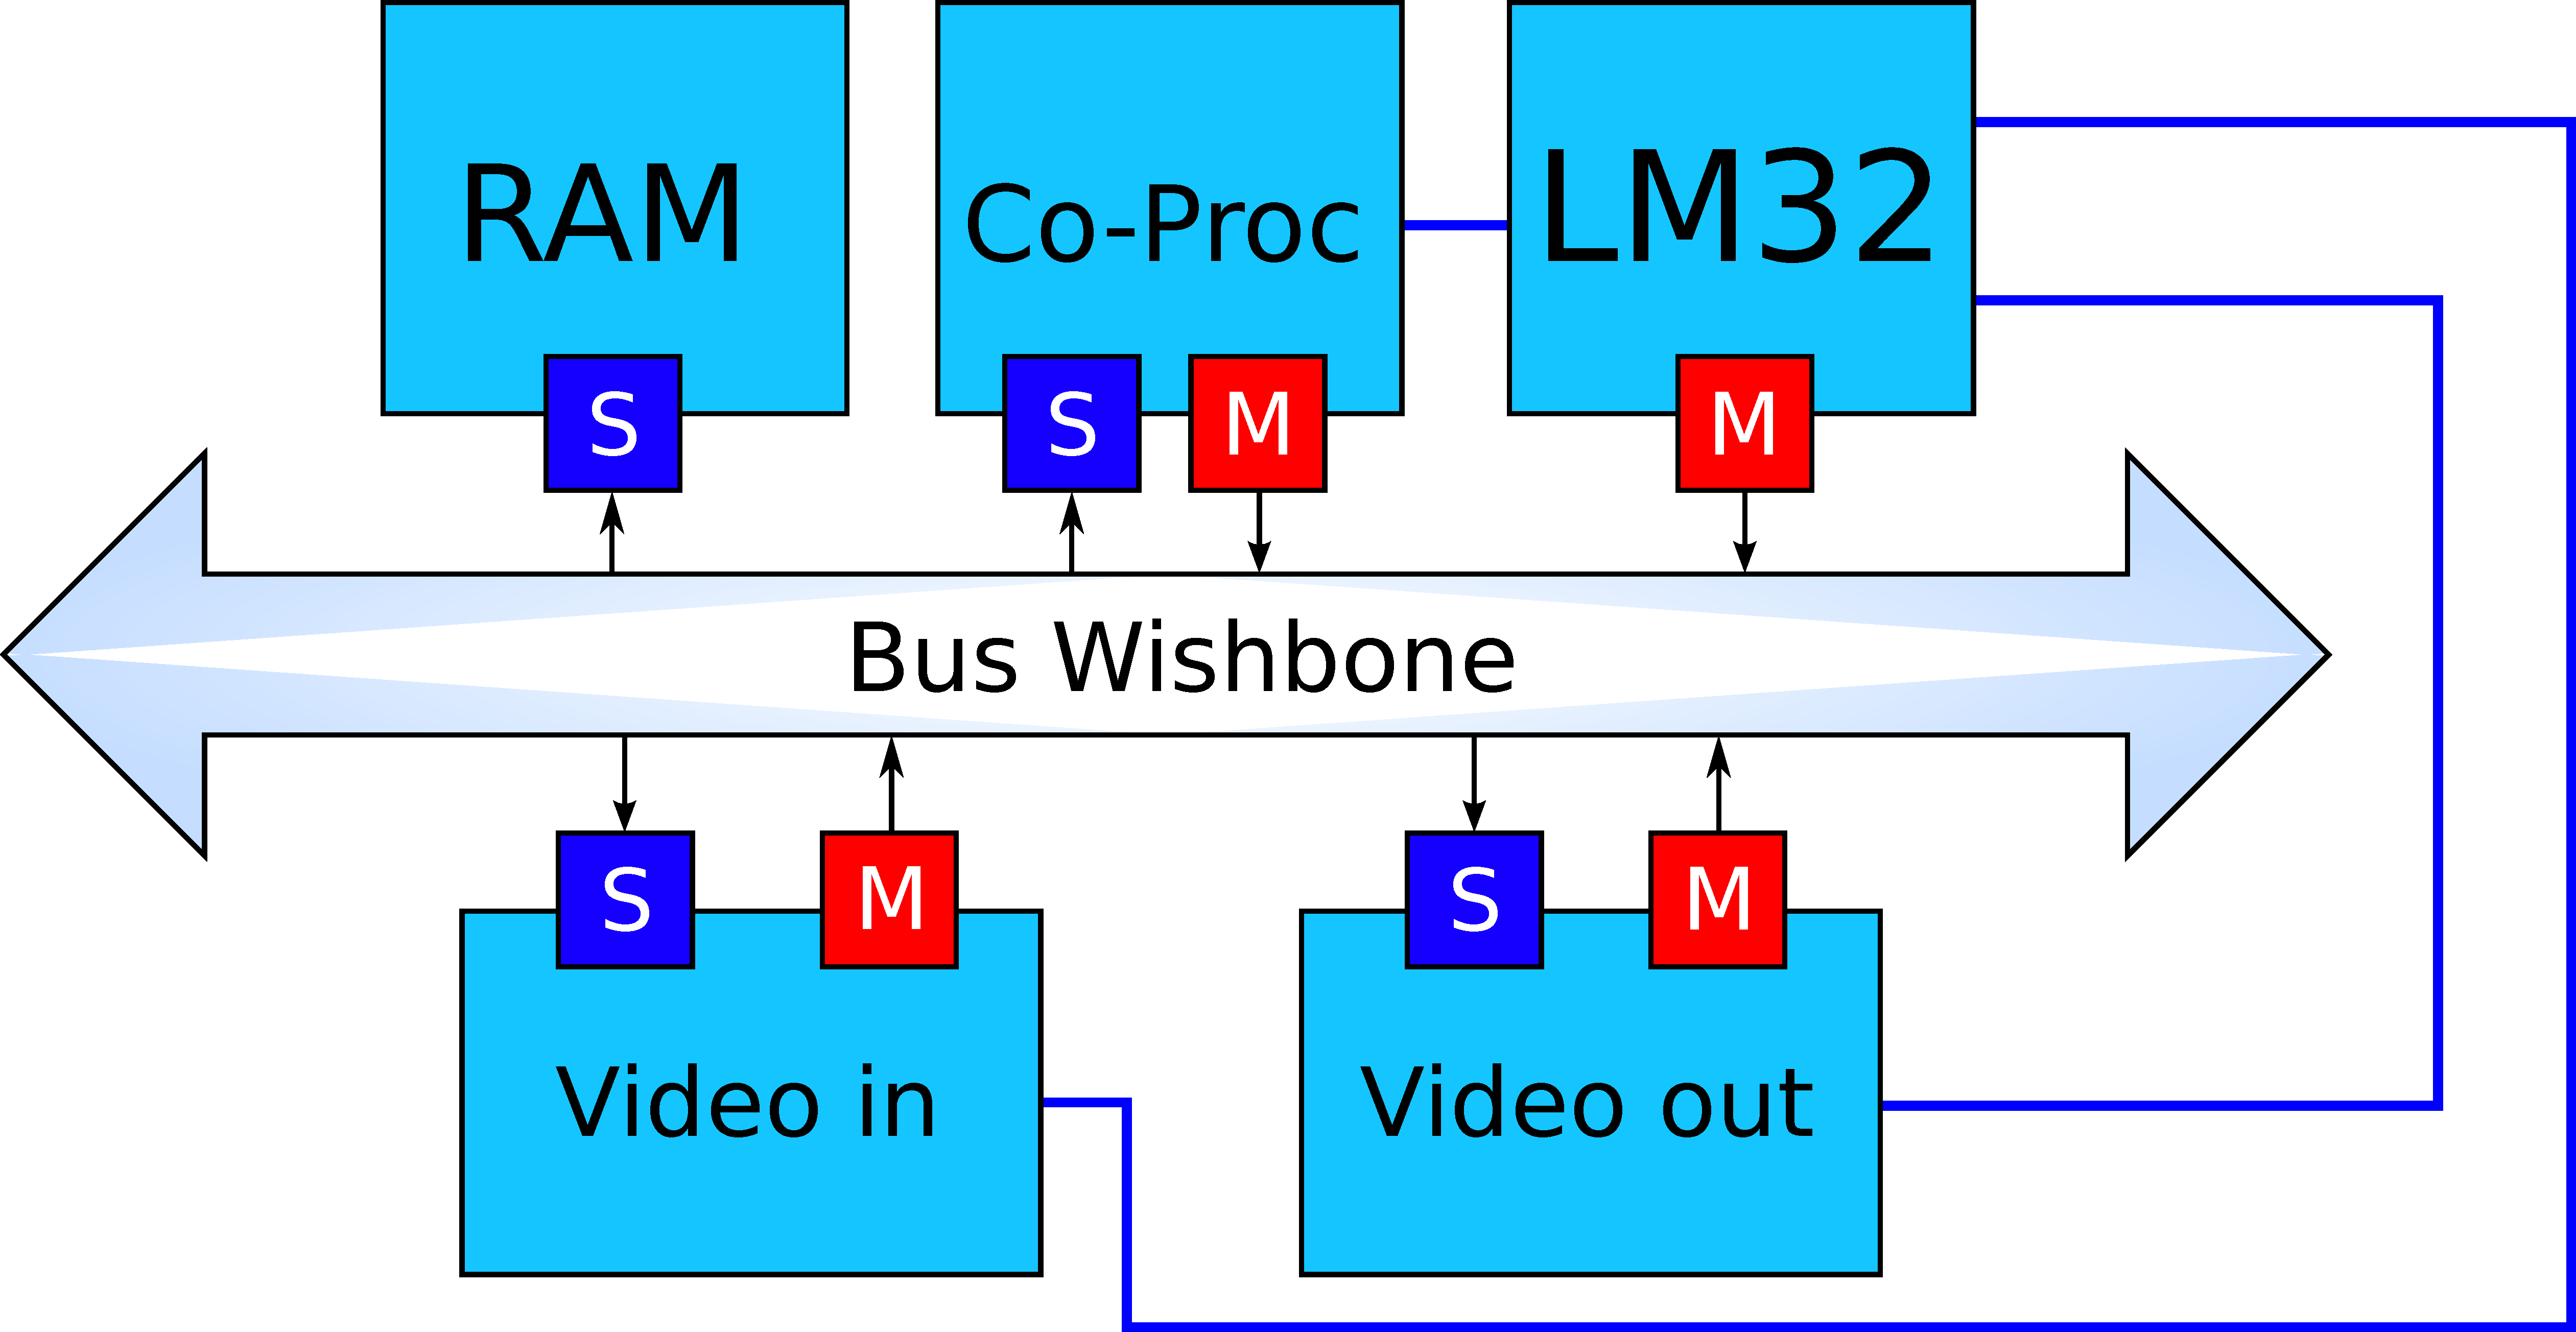
\includegraphics[width=11cm]{figs/overall_arch.pdf}

	\caption{Overall Architecture}
	\label{archi}
\end{figure}

%%%%%%%%%%%%%%%%%%%%%%%%%%%%%%%%%%%%%%%%%%%%%%%%%%%%%
%				  Video In module					%
%					-----------						%
% Author: Vaibhav Singh	& Thibault Porteboeuf 		%
%%%%%%%%%%%%%%%%%%%%%%%%%%%%%%%%%%%%%%%%%%%%%%%%%%%%%

\section{Video-In module}
\begin{figure}[H]
\center
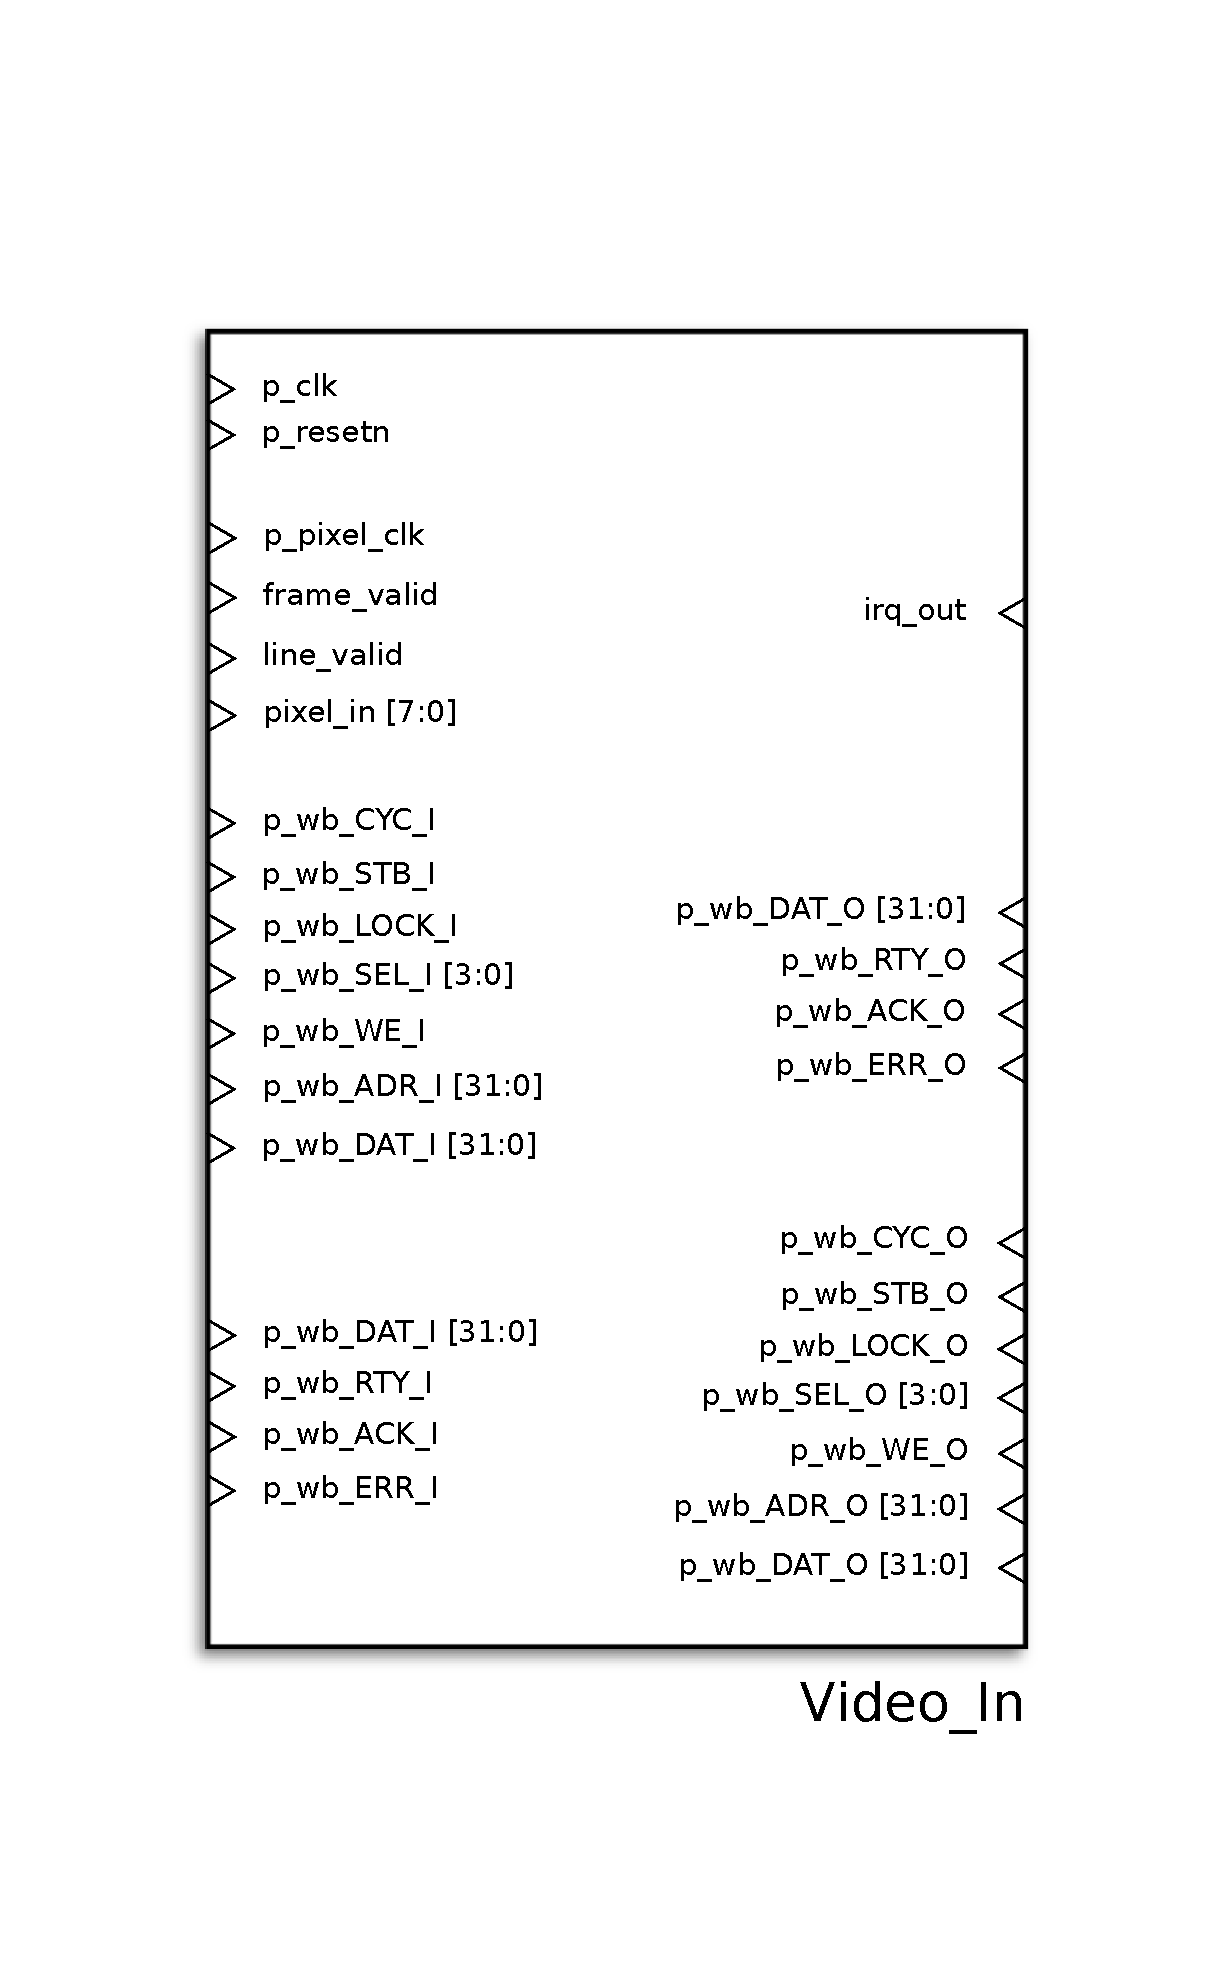
\includegraphics[width=7cm]{figs/Video_in.pdf}
\caption{Video-In module's interface}
\label{VideoIn_interface}
\end{figure}

As explained before, Video-In is the module responsible for handling the incoming video signals and transfer the pixels to the RAM over the whishbone bus.

As described in the figure below, Video In Module has a Wishbone Master Module and a one register slave, as described in section \ref{wb_reg_slave}.

Video In has two blocks, one that takes pixels from video generator running at a frequency of 25 Mhz, and an other one that stores data on to RAM. Synchronisation of internal signals between the two different clock domains has been done by sampling the 25 Mhz clock, using the system's 100 Mhz clock.

The wishbone slave will handle incoming requests from the LM32, and store the content of write requests (start address of images) to its register. It is also responsible for driving the Irq (Interrupt Request) wire which will be raised to high whenever video in requests a new start address from the LM32. The slave will automatically acknowledge when a write request is received.

The state machine samples the configuration stored in the slave's register at every rising edge of the \texttt{frame\_valid} signal. Thus, the configuration is updated only at the beginning of a new frame.

It then posts data from the buffer to the RAM, starting at the previously given address. This process is illustrated in figure \ref{VideoIn_sm}. 

It is important to notice that, following the idea that the peripherals are driven and configured by the LM32, the VideoIn module will remain Idle until the LM32 activates it by carrying a first write request to VideoIn's slave.

Detailed explanation of video in can be found along the explanation of the source code.

\begin{figure}[h]
\center
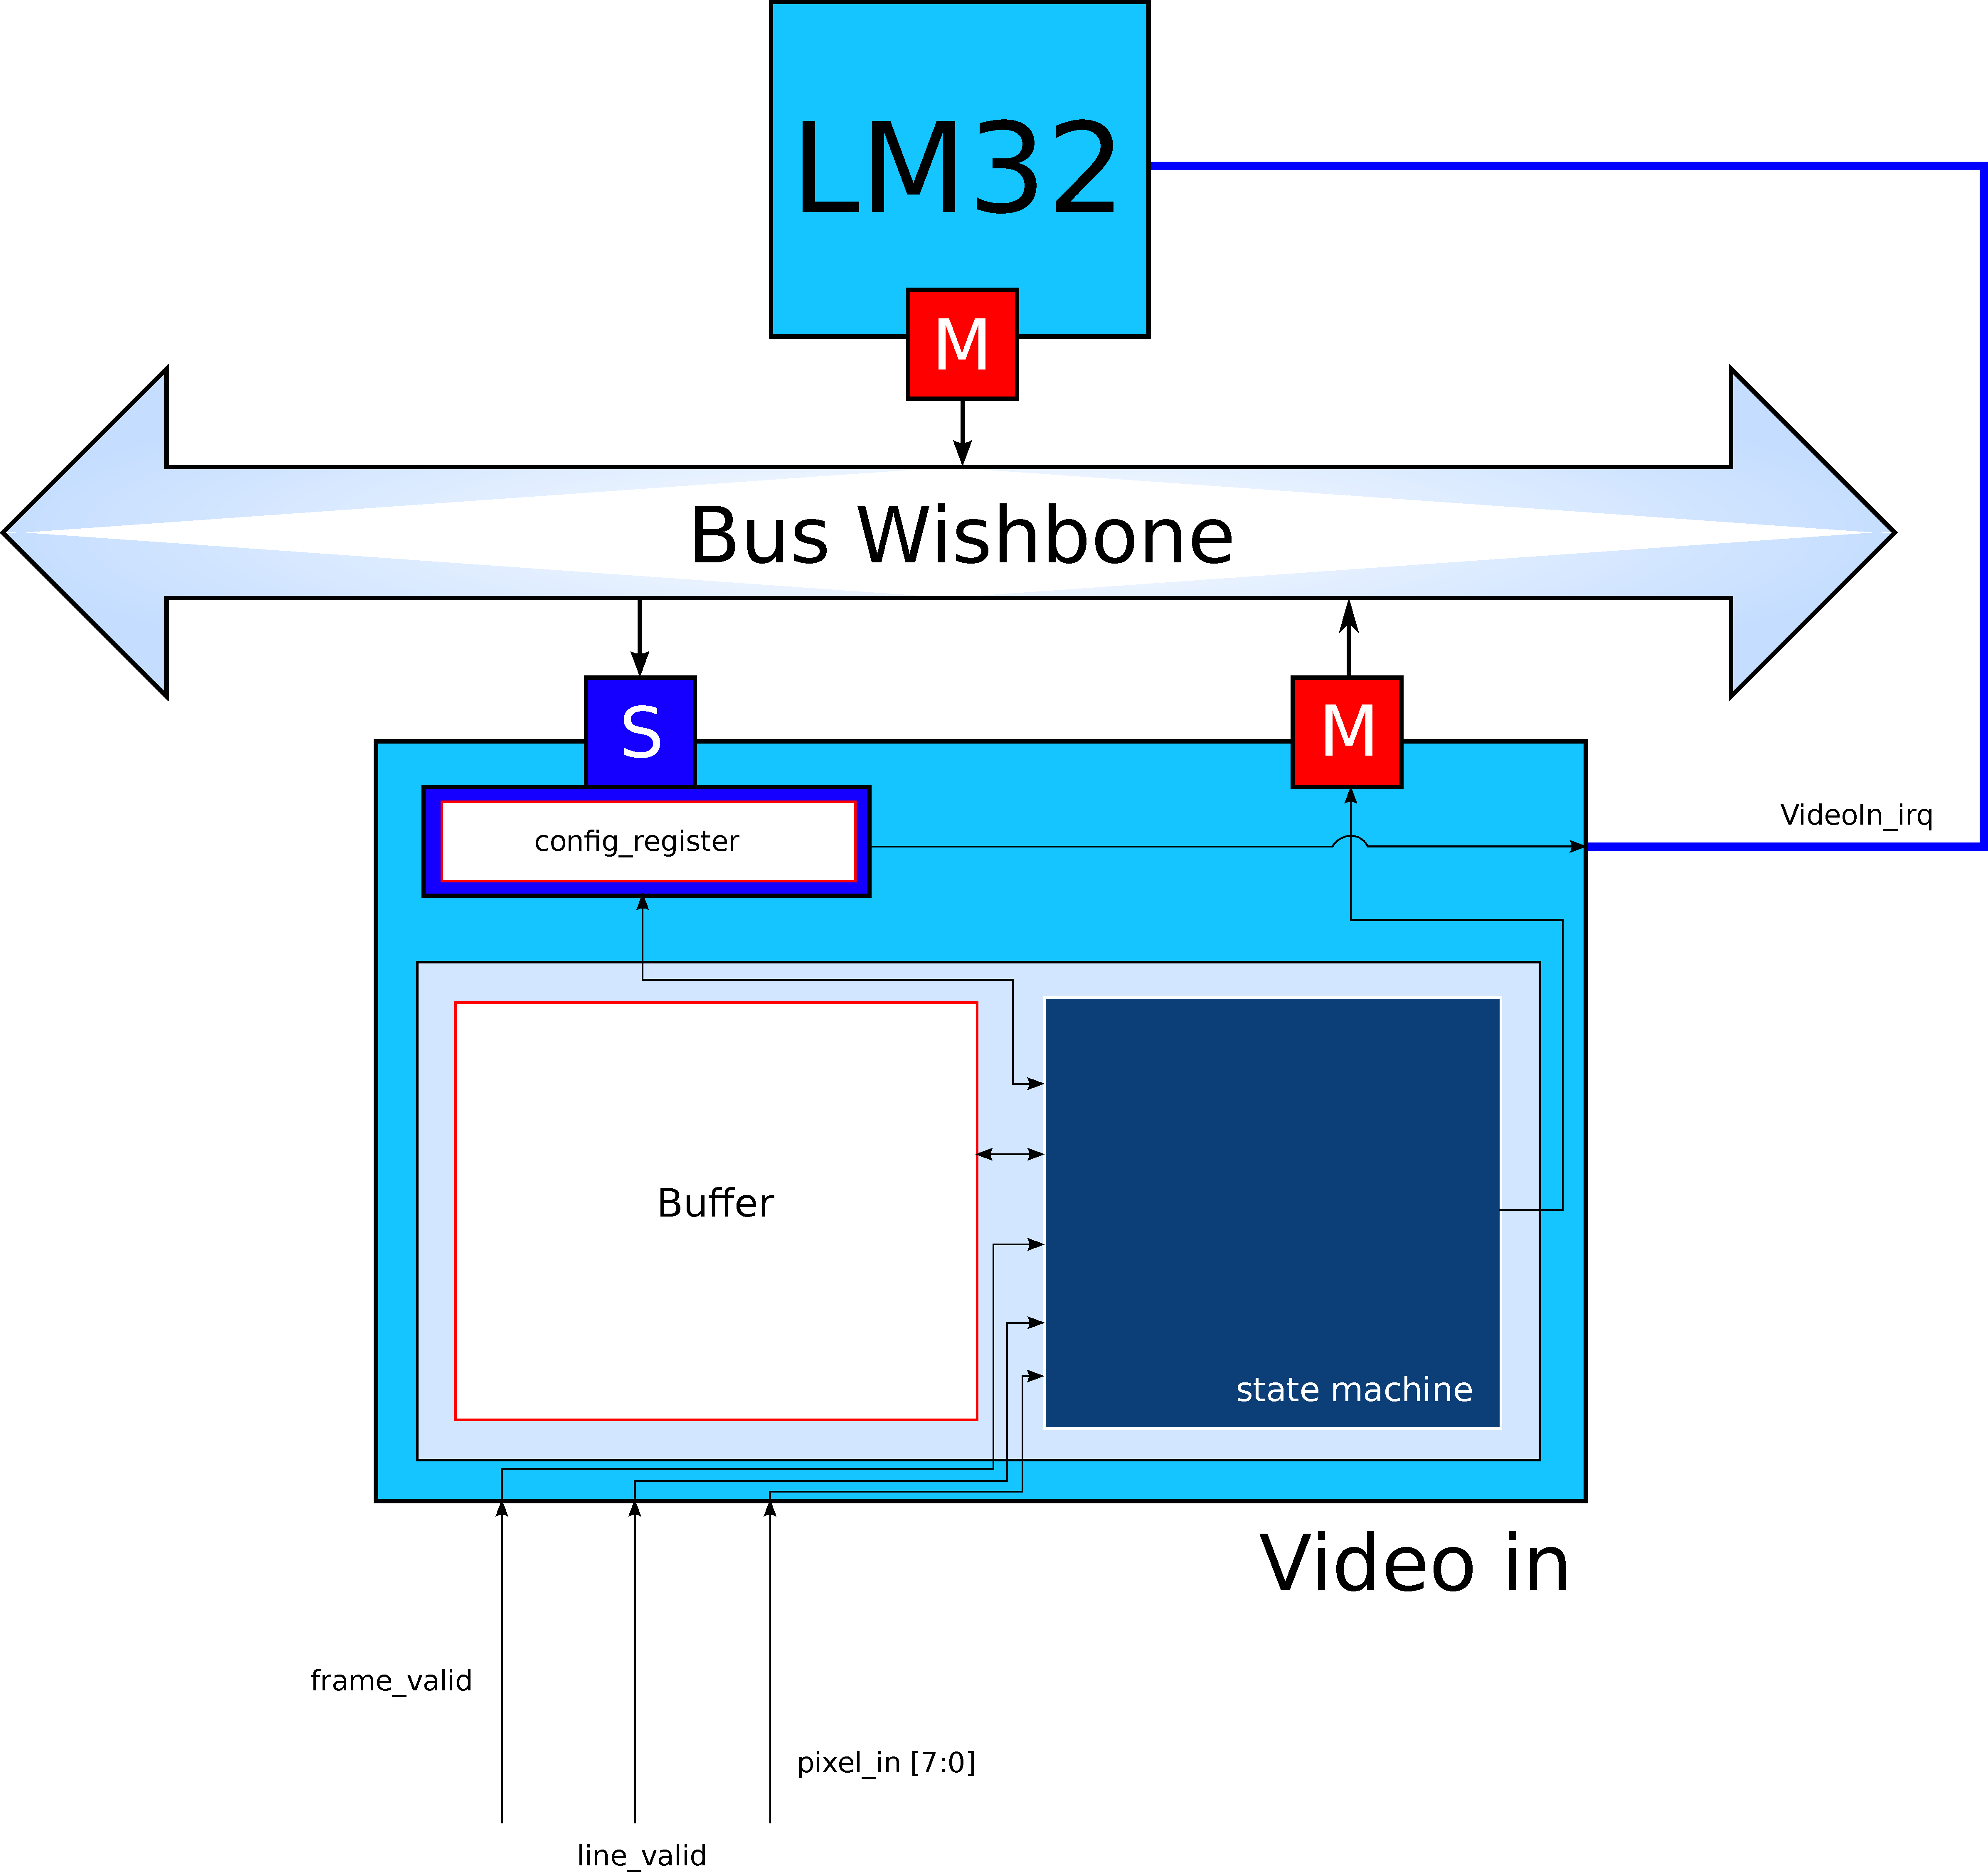
\includegraphics[width=11cm]{figs/Video_In_blocks.pdf}
\caption{VideoIn's inner structure}
\label{VideoIn_struct}
\end{figure}


\begin{figure}[h]
\center
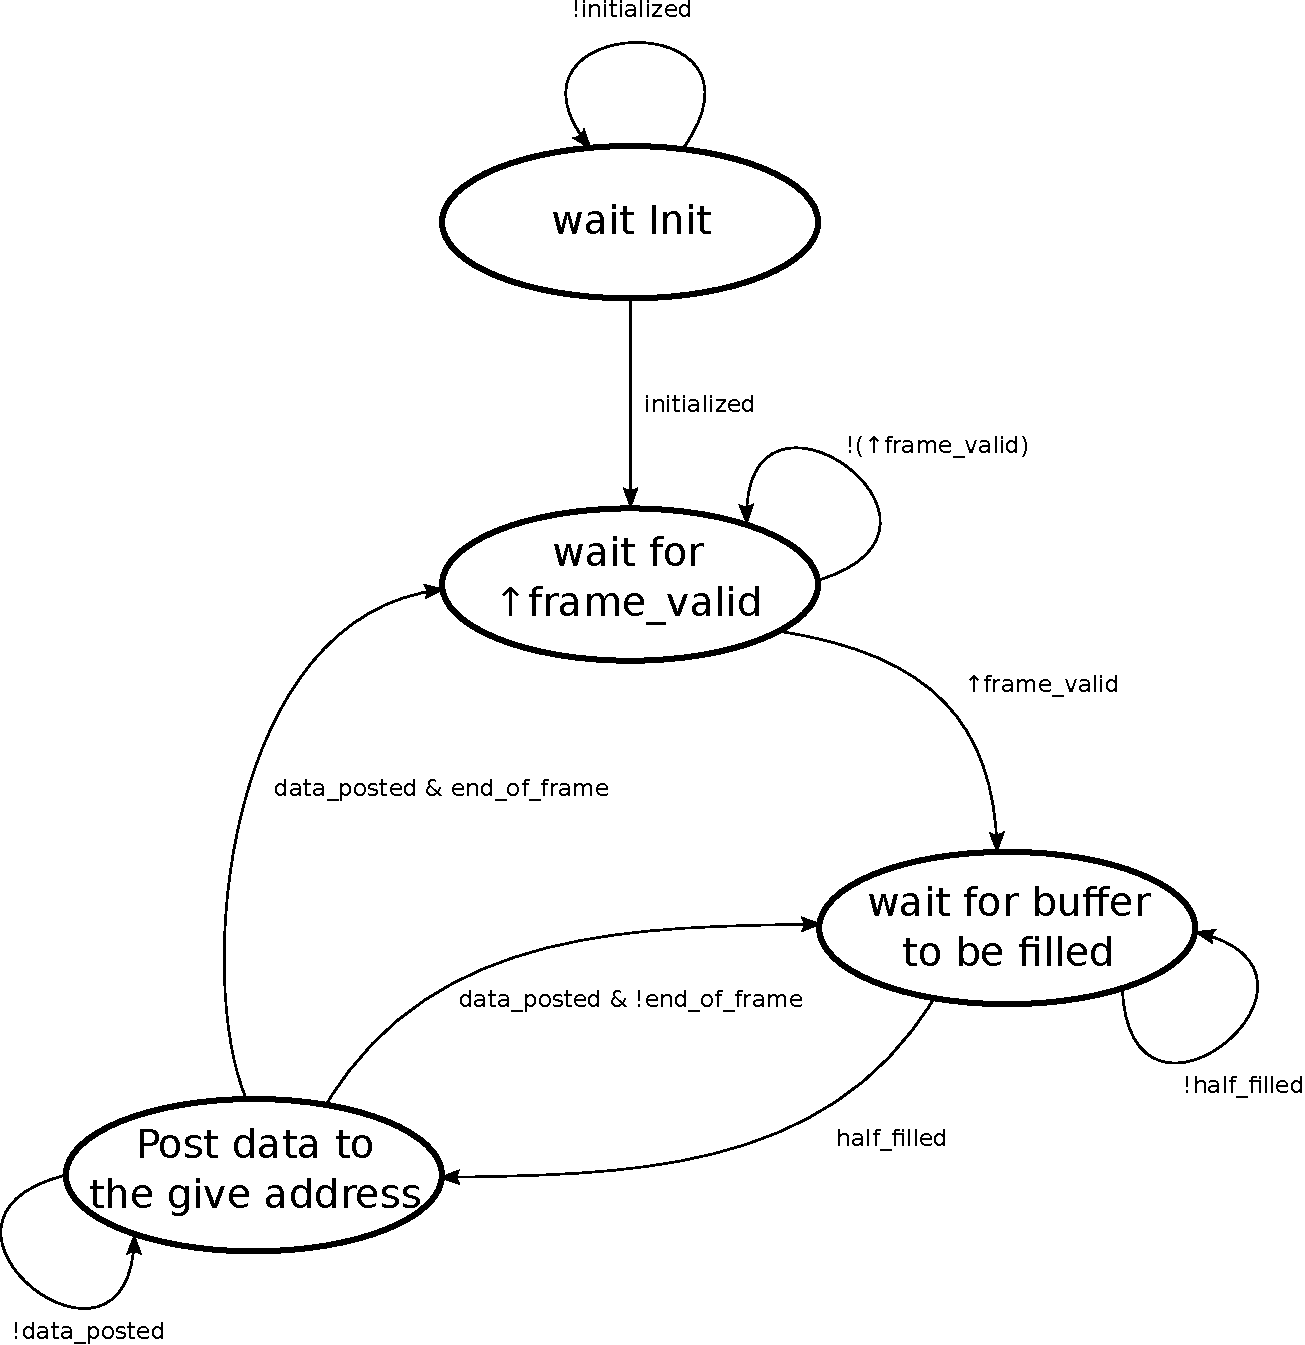
\includegraphics[width=11cm]{figs/video_in_sm.pdf}
\caption{VideoIn's behavior}
\label{VideoIn_sm}
\end{figure}


%%%%%%%%%%%%%%%%%%%%%%%%%%%%%%%%%%%%%%%%%%%%%%%%%%%%%
%			      Video Out module					%
%					-----------						%
% Author: Thibault Porteboeuf						%
%%%%%%%%%%%%%%%%%%%%%%%%%%%%%%%%%%%%%%%%%%%%%%%%%%%%%

\section{Video-Out module}

\begin{figure}[H]
\center
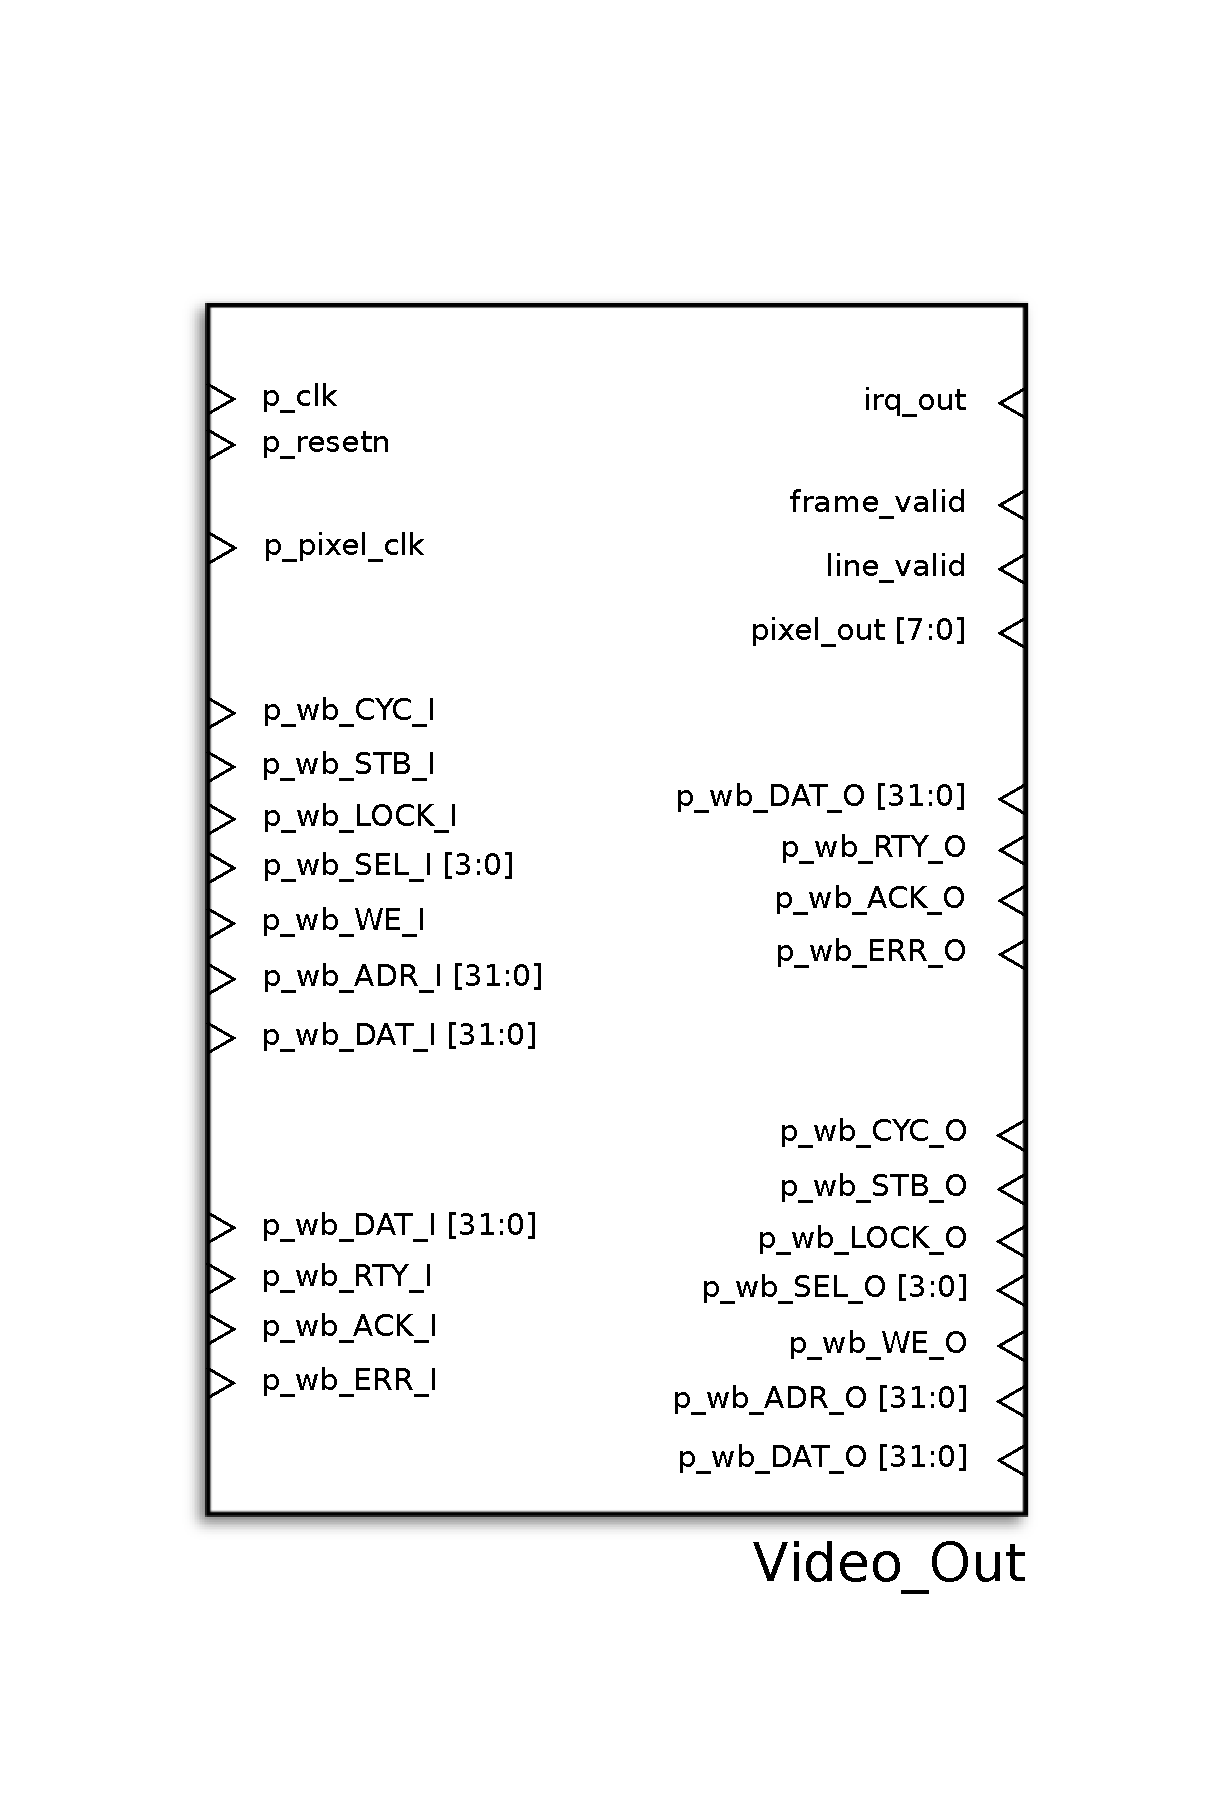
\includegraphics[width=7cm]{figs/Video_out.pdf}
\caption{VideoOut module's interface}
\label{VideoOut_interface}
\end{figure}

The Video-Out module, in design, is similar to the VideoIn module, as presented in figure \ref{VideoOut_struct}. It also has a one register slave module presented in section \ref{wb_reg_slave} and a wishbone master interface.


Video-Out is responsible to read the pixels stored on the ram and output it to the video display module.

The different ports are detailed in figure \ref{VideoOut_interface}.

The module's behavior is described in the figure \ref{VideoOut_behavior}, and is enumerated as follows:
\begin{enumerate}
\item Video-Out remains Idle until an address to read to has been written to its slave interface by LM32, as VideoIn does.
\item When this first configuration has been set, VideoOut starts pre-loading its internal buffer.
\item Video-Out starts generating the video signals and pixels while reading from the internal buffer 
\item Each time one block of buffer has been outputted to the display module, a read request is send over the wishbone bus by VideoOut's master interface, in order to retrieve more data. Care has been taken to ensure that write operations to the buffer are always one block ahead of read operations from the buffer.
\item This process continues until the end of the image, which pauses the module. It then raises an Irq in order to get the next address to read to, and starts over.
\end{enumerate}

Here again, the one register slave module is responsible for driving the Irq wire.
The state machines asks for an Irq to be raised, and the slave automatically acknowledges it once a write request has been received from the bus. In the verilog code,video in and video out instantiate this common slave module.

\vfill
\begin{figure}[h]
\center
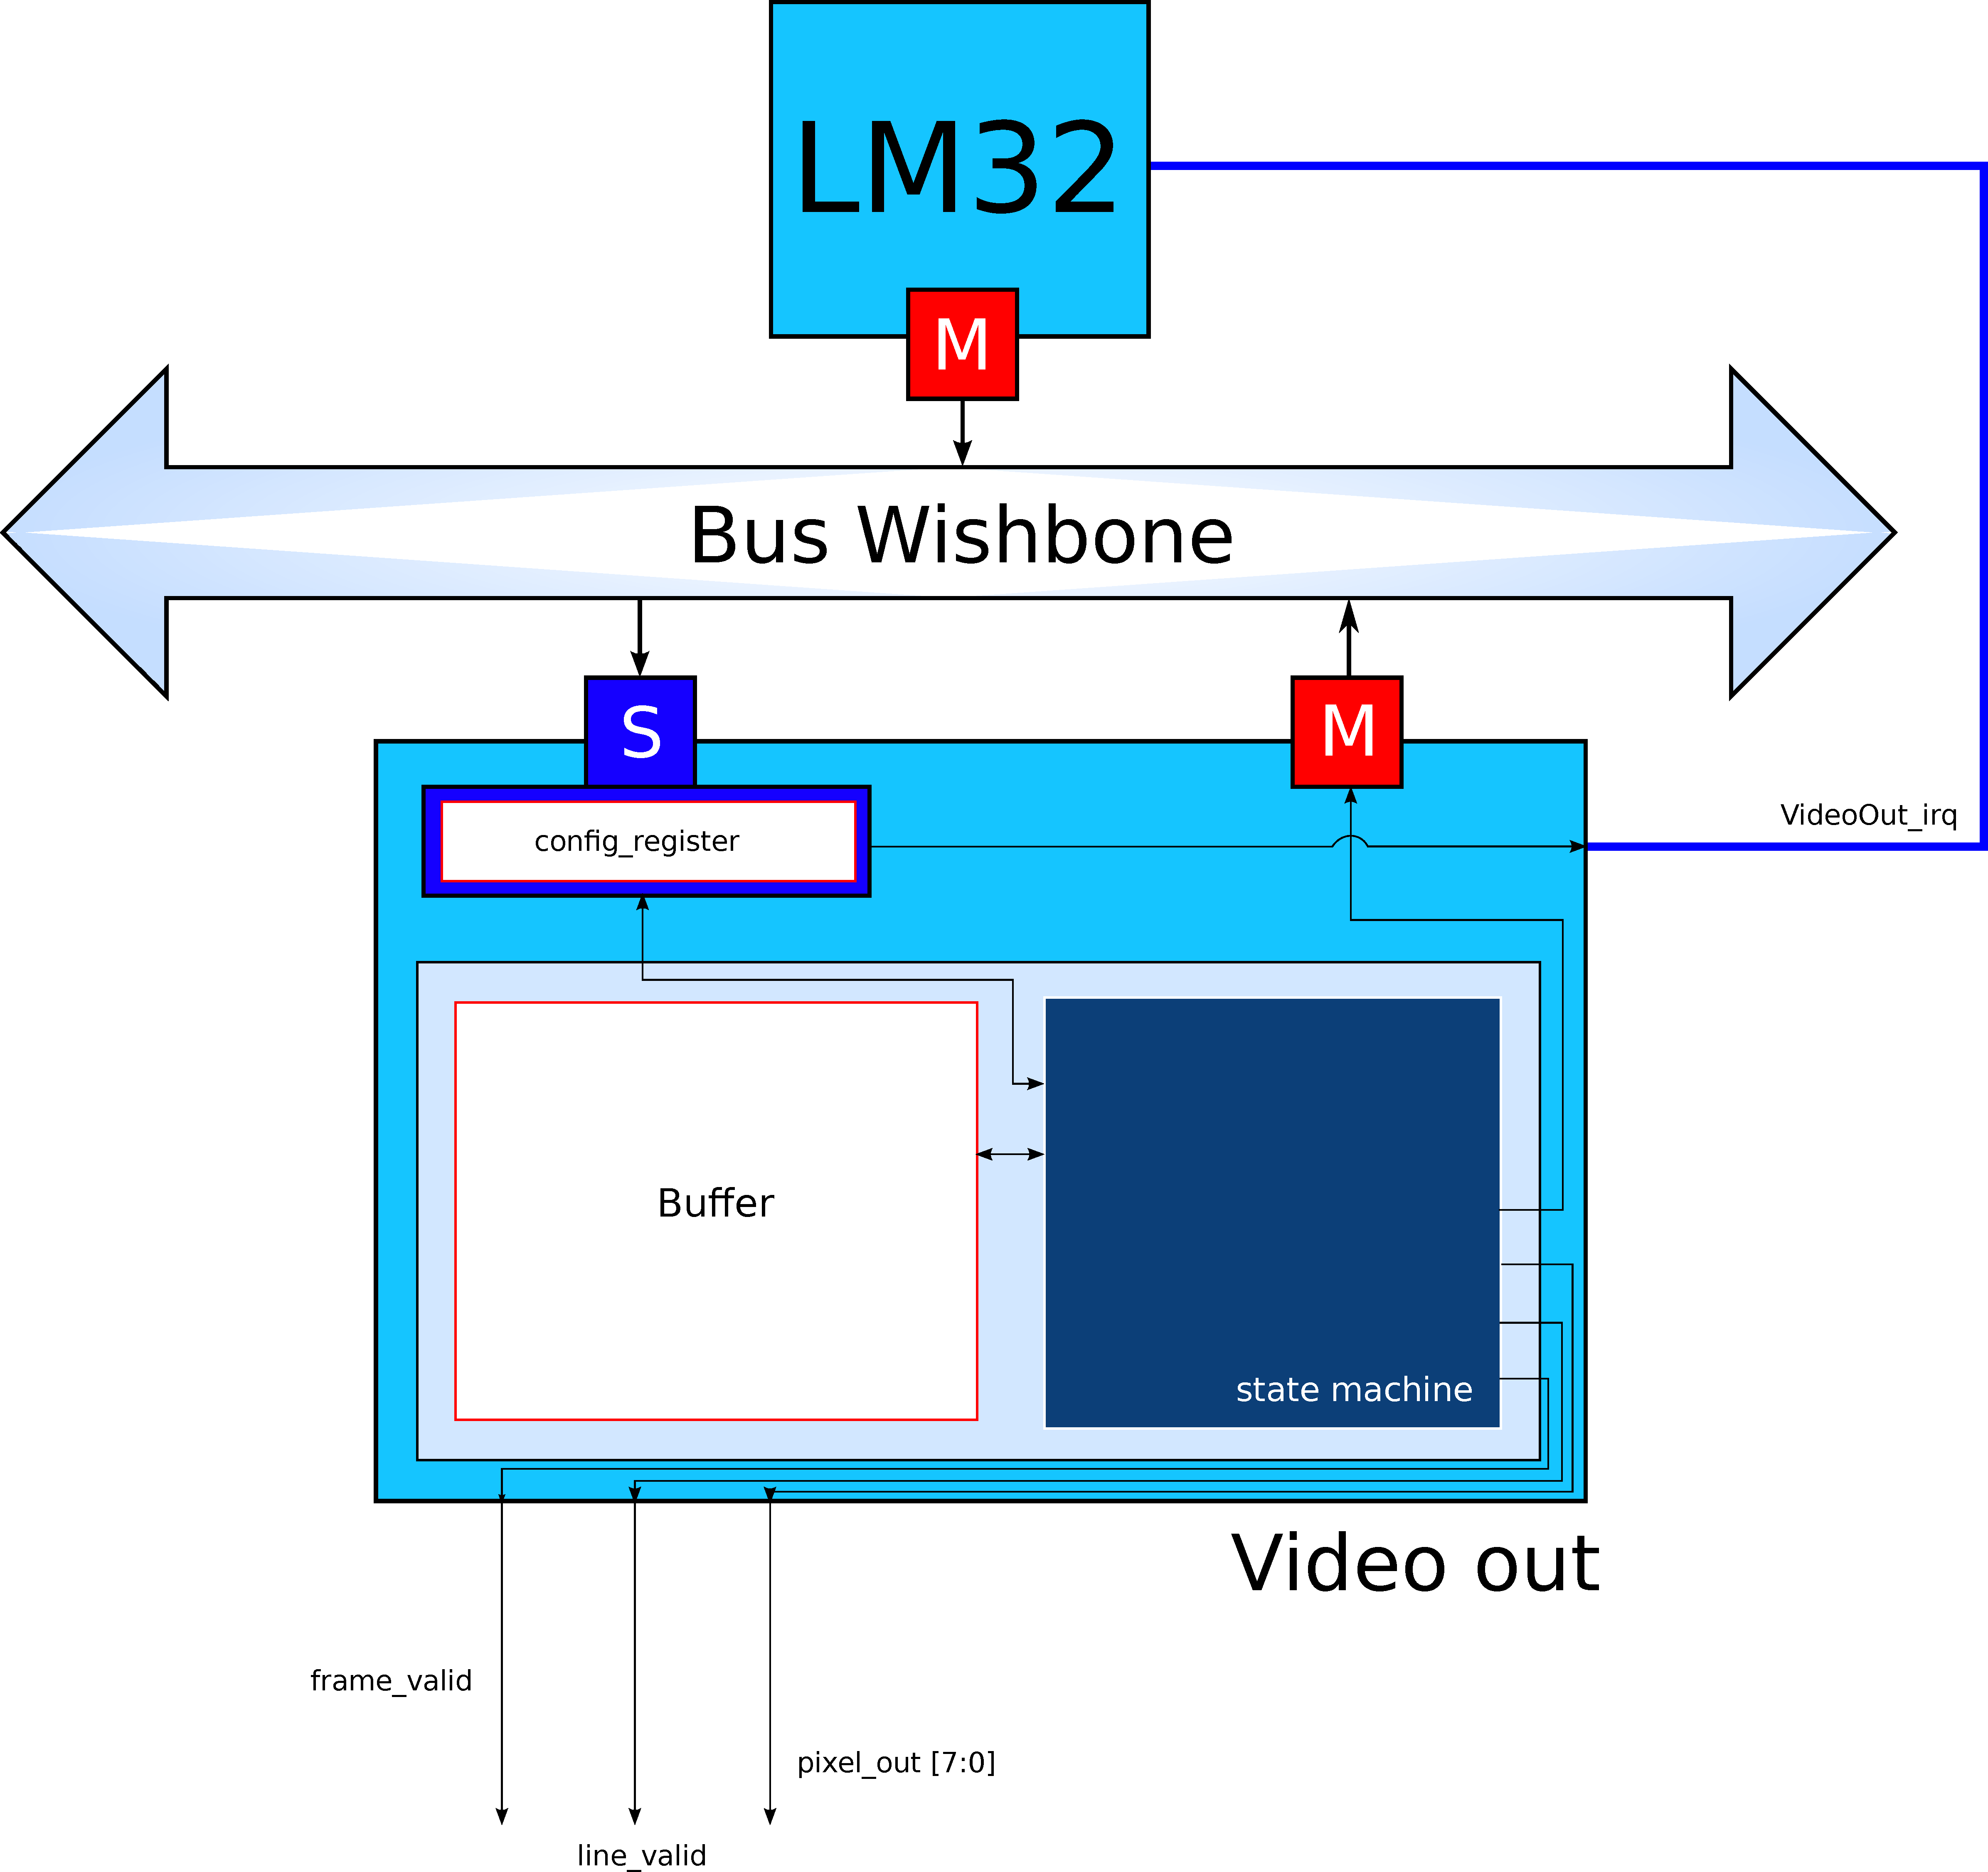
\includegraphics[width=11cm]{figs/Video_Out_blocks.pdf}
\caption{VideoOut's inner structure}
\label{VideoOut_struct}
\end{figure}
\vfill

\begin{figure}[h]
\center
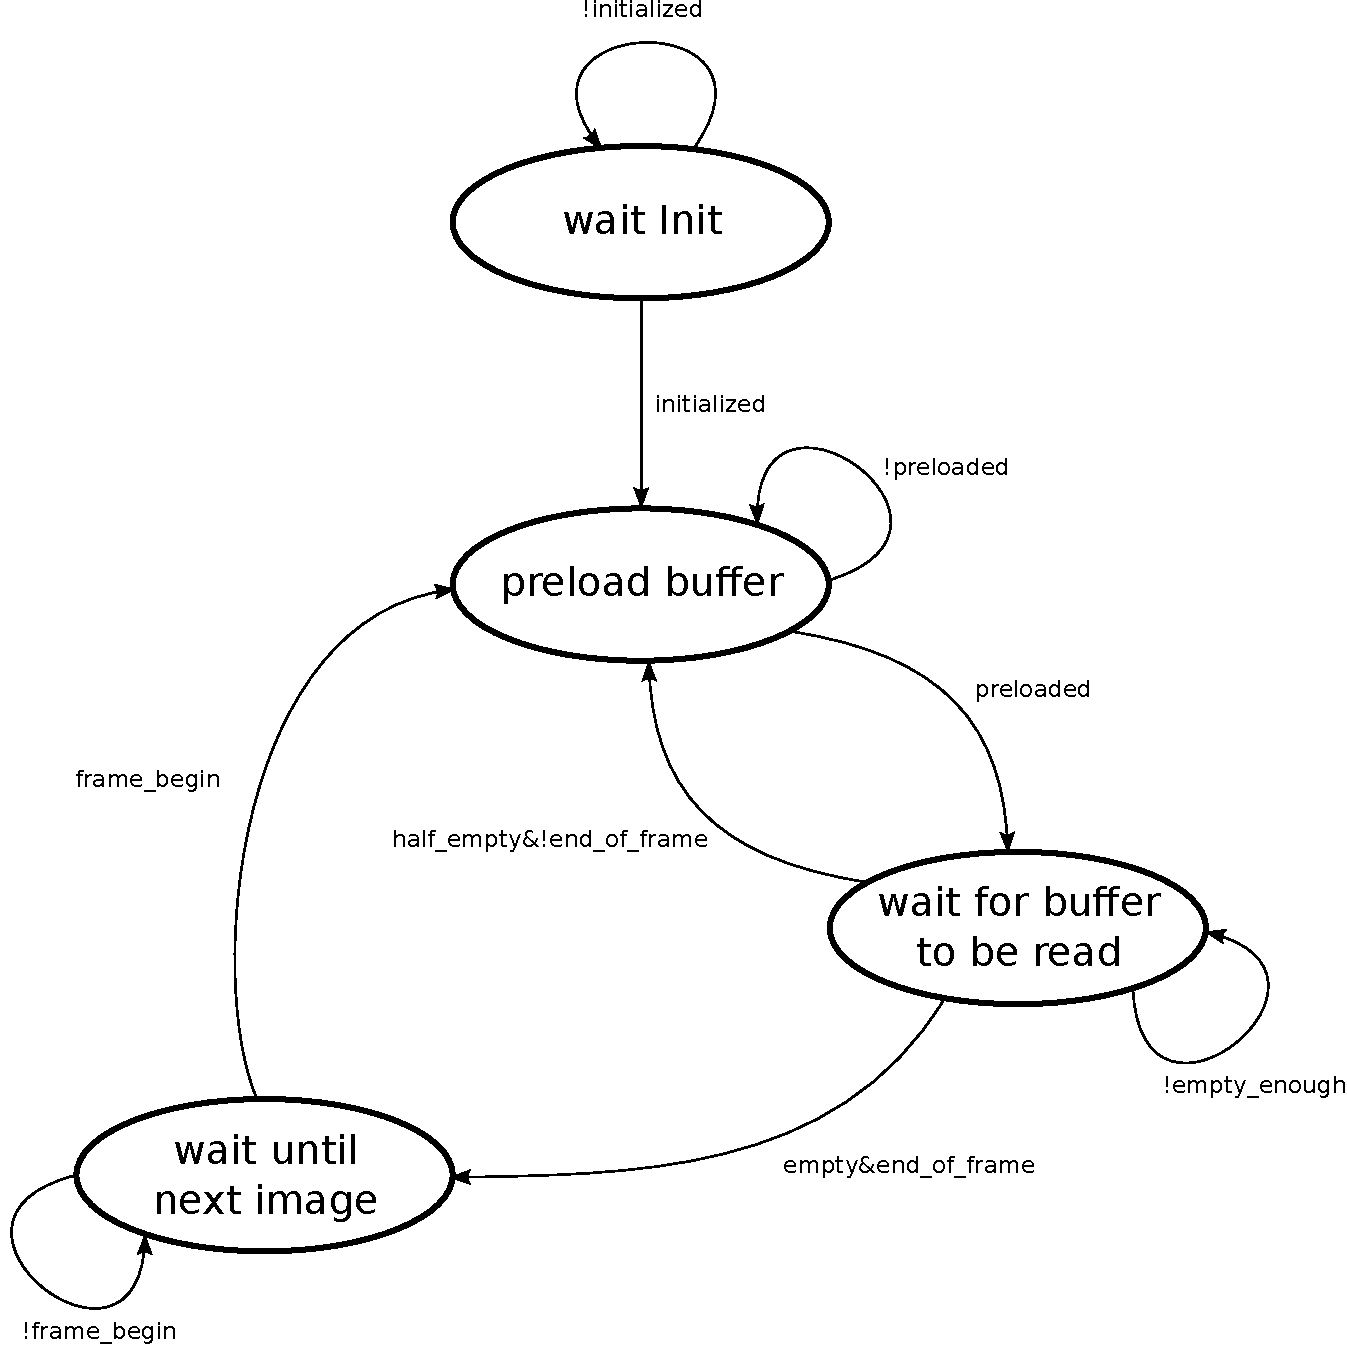
\includegraphics[width=11cm]{figs/video_out_sm.pdf}
\caption{VideoOut's behavior}
\label{VideoOut_behavior}
\end{figure}


%%%%%%%%%%%%%%%%%%%%%%%%%%%%%%%%%%%%%%%%%%%%%%%%%%%%%
%				 Coprocessor module					%
%					-----------						%
% Author: Theodoros Theodoropoulos&Adrian Schindler %
%%%%%%%%%%%%%%%%%%%%%%%%%%%%%%%%%%%%%%%%%%%%%%%%%%%%%


\section{Coprocessor}


The following section describes the inner structure of the coprocessor.

It comprises a subsection regarding the incremental calculation module, and subsections regarding the buffer management and the interpolation.

\begin{figure}[h]
\center
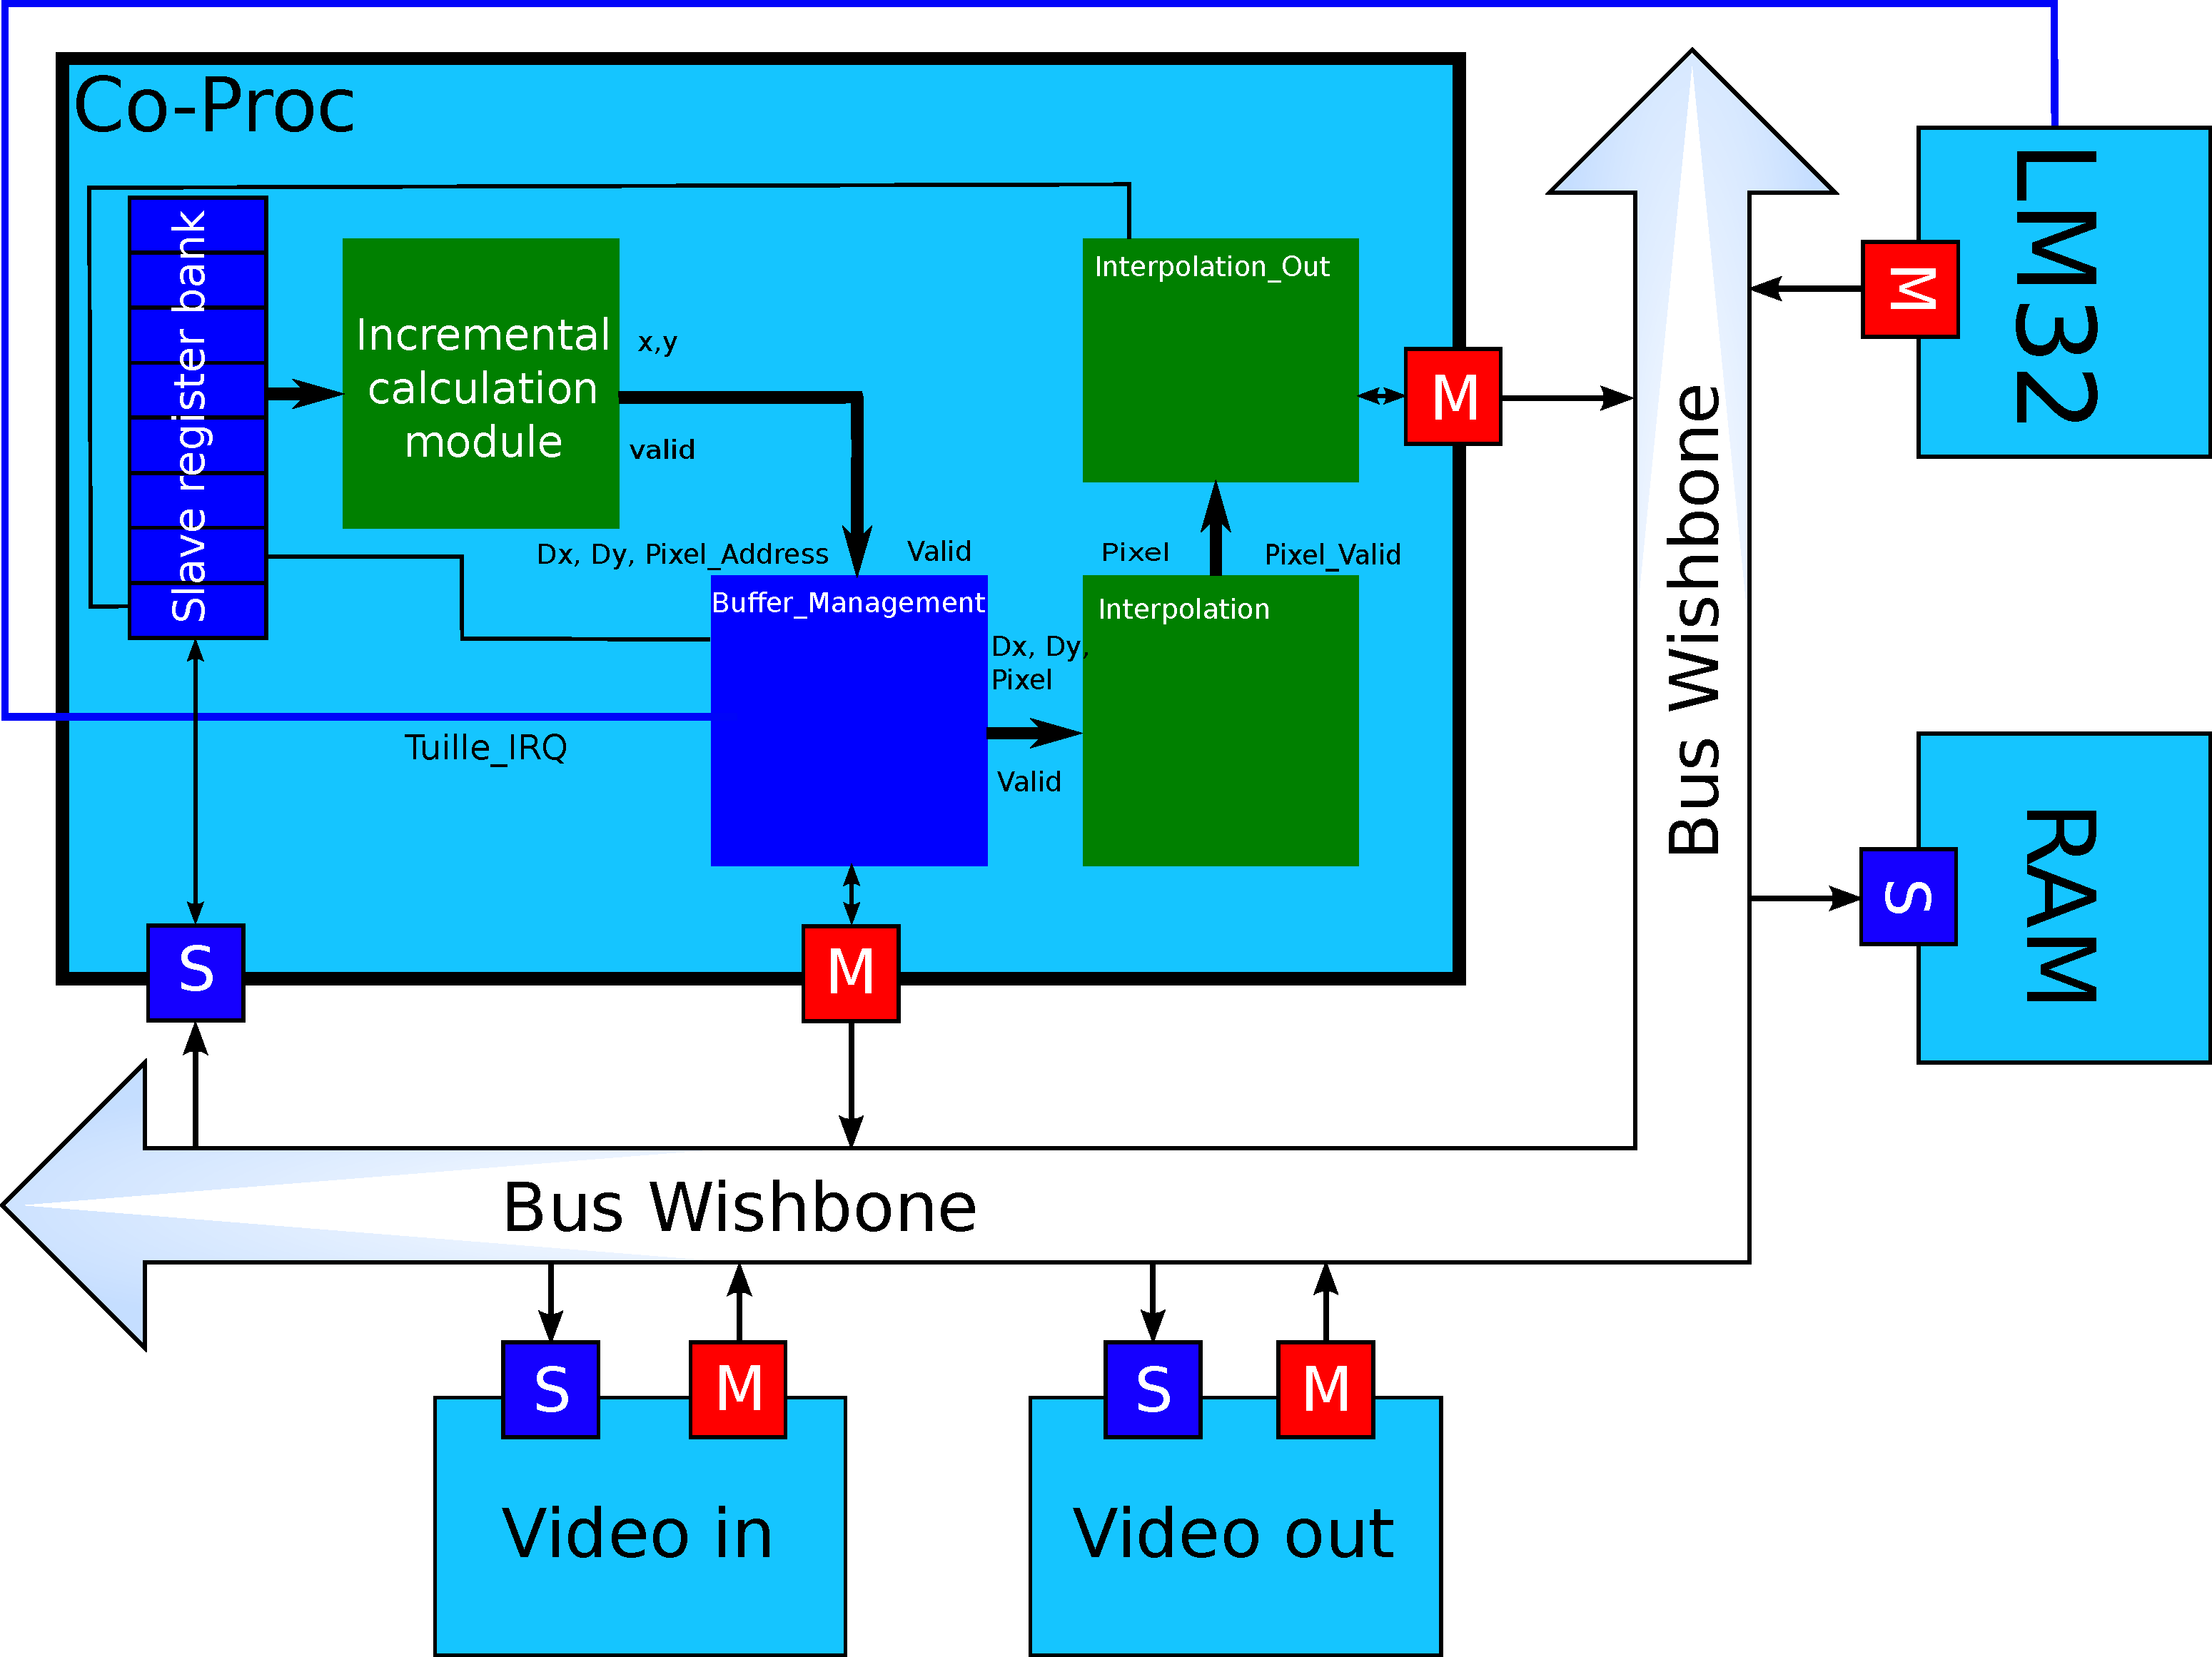
\includegraphics[width=11cm]{figs/copro2.pdf}
\caption{Coprocessor's inner structure}
\label{coproc_struct}
\end{figure}

\subsection{Calculation module}

\subsubsection{Incremental module}

\begin{figure}[H]
\center
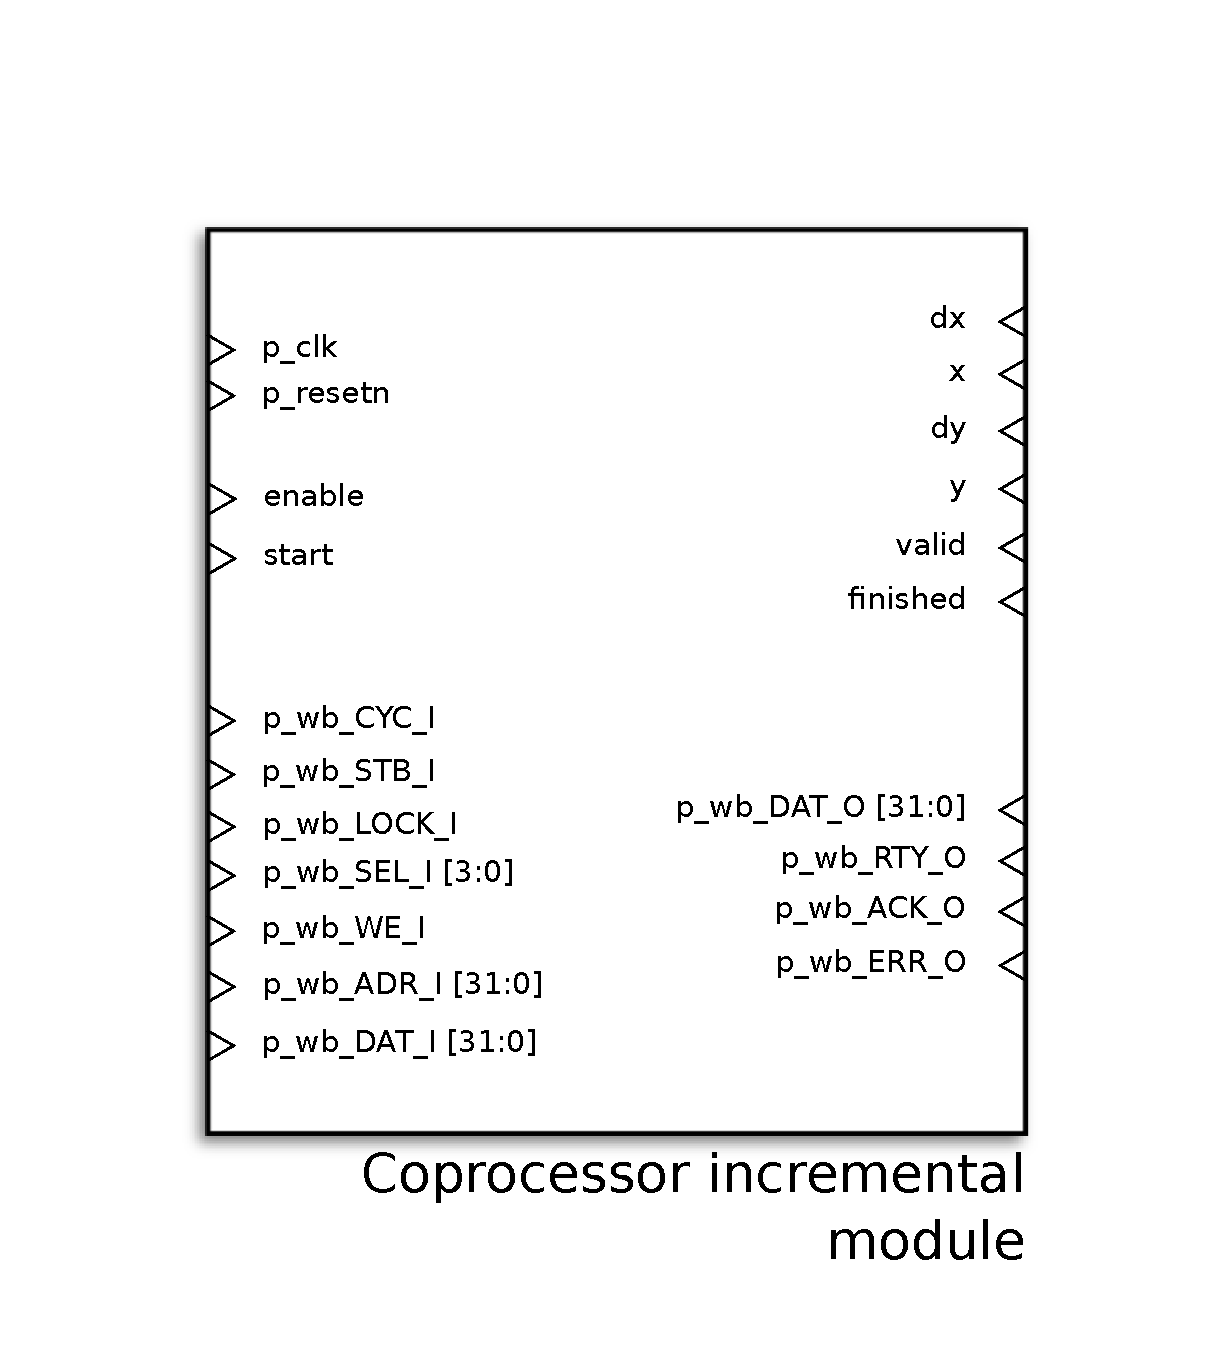
\includegraphics[width=7cm]{figs/coproc_incr_symbol.pdf}
\caption{Coprocessor incremental calculation module's input/output ports}
\label{Incr_interface}
\end{figure}


The incremental calculation module consists of one clock-triggered process. Unlike other modules which work on an entire image it works on a tile-by-tile basis: It loads the coefficients for the new tile and then outputs the 16 x 16 pixels. Data is stored in the mfixed format, however, the version provided on the SEN website (\url{http://sen.enst.fr/ue/elec342/v_fixe}) has been modified to be C++ compatible and work with SystemC. We transformed the C union into a class with two private values which can be extracted by two public functions; in line with object-oriented programming concepts. For ease of use, we also added the + and \= operator which internally use fx\_add and fx\_copy. In addition, we added functions for debug purposes: the \texttt{<}\texttt{<} operator for command line output and sc\_trace for signal tracing.

The functionality of the module can be enabled/disabled via the \texttt{enable} signal. This does also work in the middle of a calculation, for instance during the calculation process of a tile. There are three states which are traversed during the calculation of any tile illustrated in figure \ref{incr_sm} and enumerated as follows:

\begin{itemize}
\item State 0: If the start signal is high, the coefficients are loaded from the wishbone slave interface (which have been written there by the LM32 beforehand) to an internal register for each coefficient. We had to typecast the uint32\_t value output by the wishbone interface to mfixed which does not cause any problem since the upper portion of the mfixed type (which represents the digit) is unsigned. Once the start signal passes to low, the calculation will begin and the module passes to state 1.
\item State 1: In this state, the coprocessor outputs one pixel per clock cycle. It indicates this by the valid signal which is high during the whole tile calculation. The calculation process follows the incremental calculation suggested by Pacalet (\url{http://sen.enst.fr/filemanager/active?fid=326}) and therefore only consists of additions. These are performed on the internal registers. An internal counter keeps track of the number of pixels processed. After the last pixel of the tile, the coprocessor passes to state 2.
\item State 2: The Coprocessor remains in this state for one cycle and sets the finished signal high for one clock cycle to indicate that the last pixel has been processed; at the same time the valid signal is set low. Then, the coprocessor automatically passes to state 0.

\end{itemize}
\begin{figure}[H]
\center
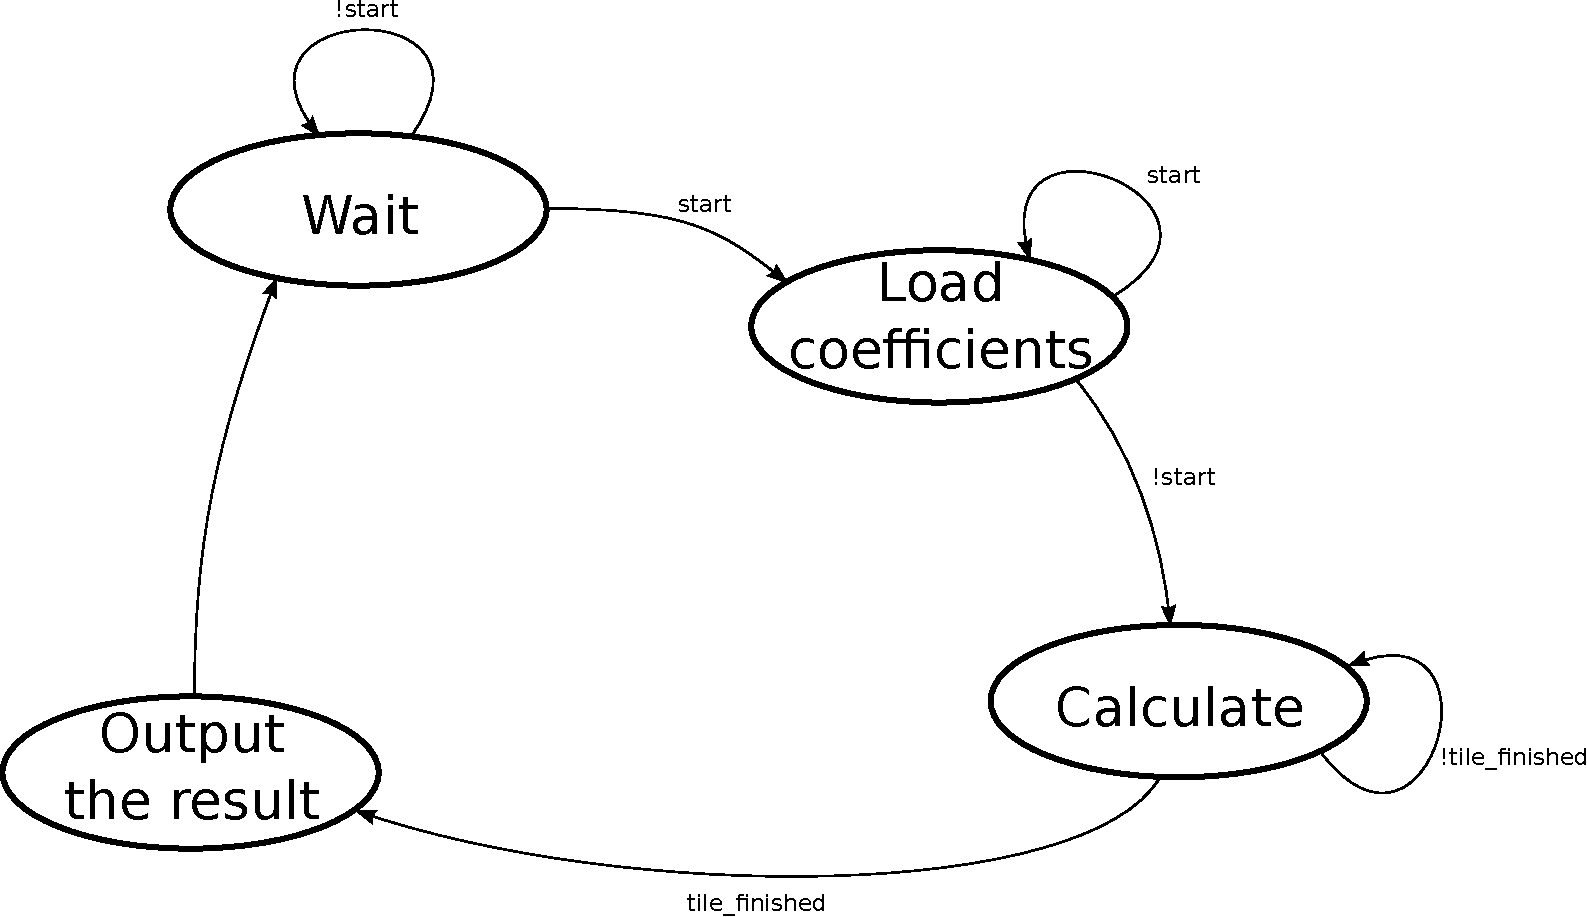
\includegraphics[width=11cm]{figs/coproc_incr_sm.pdf}
\caption{Coprocessor incremental calculation state machine}
\label{incr_sm}
\end{figure}

The module outputs both the x- and y-coordinates by the means of two processes running in parallel. In the slave module, the y-coordinates are stored with an address offset of 40, and two separate sets of internal registers are allocated. Therefore, no conflicts can occur.

To test the operation of the incremental calculation module, we have written a dedicated test-bench in SystemC which uses a formula to calculate the output x-coordinate directly for a given x and y output coordinates and coefficients. We initialised the Coprocessor thanks to a function which calculated the coefficients to be used by the incremental calculation module. This already allowed us to verify the functionality of the formulas using the mfixed type. It was sufficient to test the x-coordinate only since both the x and y coordinate follow the same principle. In particular, we used it to verify that the error between expected and observed value was not greater than 3\%; a value we judged acceptable. Errors are introduced due to the incremental calculation formula itself as well as the truncation in the mfixed format.

\subsubsection{Module's configuration: multiple register slave}



The configuration is transmitted to the module using a wishbone slave including multiple registers.
The coefficient slave has 20 internal registers to buffer the values calculated by the LM32 (10 for the x and 10 for the y coordinates) until they are accessed by the incremental calculation module. The module uses two internal registers: If 20 coefficients have been written, the ready signal is set high. This indicates the coprocessor that it can load these and start its calculations. In any case, all 20 coefficients must be set in a burst, i.e. writing to one register will set the ready signal down automatically until all 20 coefficients have been written. Nevertheless, no effort has been made to verify that 20 different registers have been written to and the responsibility lies with the LM32. Similarly, the internal loaded register indicates if 20 reads have been performed. The objective is to inform the LM32 if the coefficients have been loaded by the coprocessor and can thus be overwritten by new ones.

\subsection{Interpolator}

\begin{figure}[H]
\center
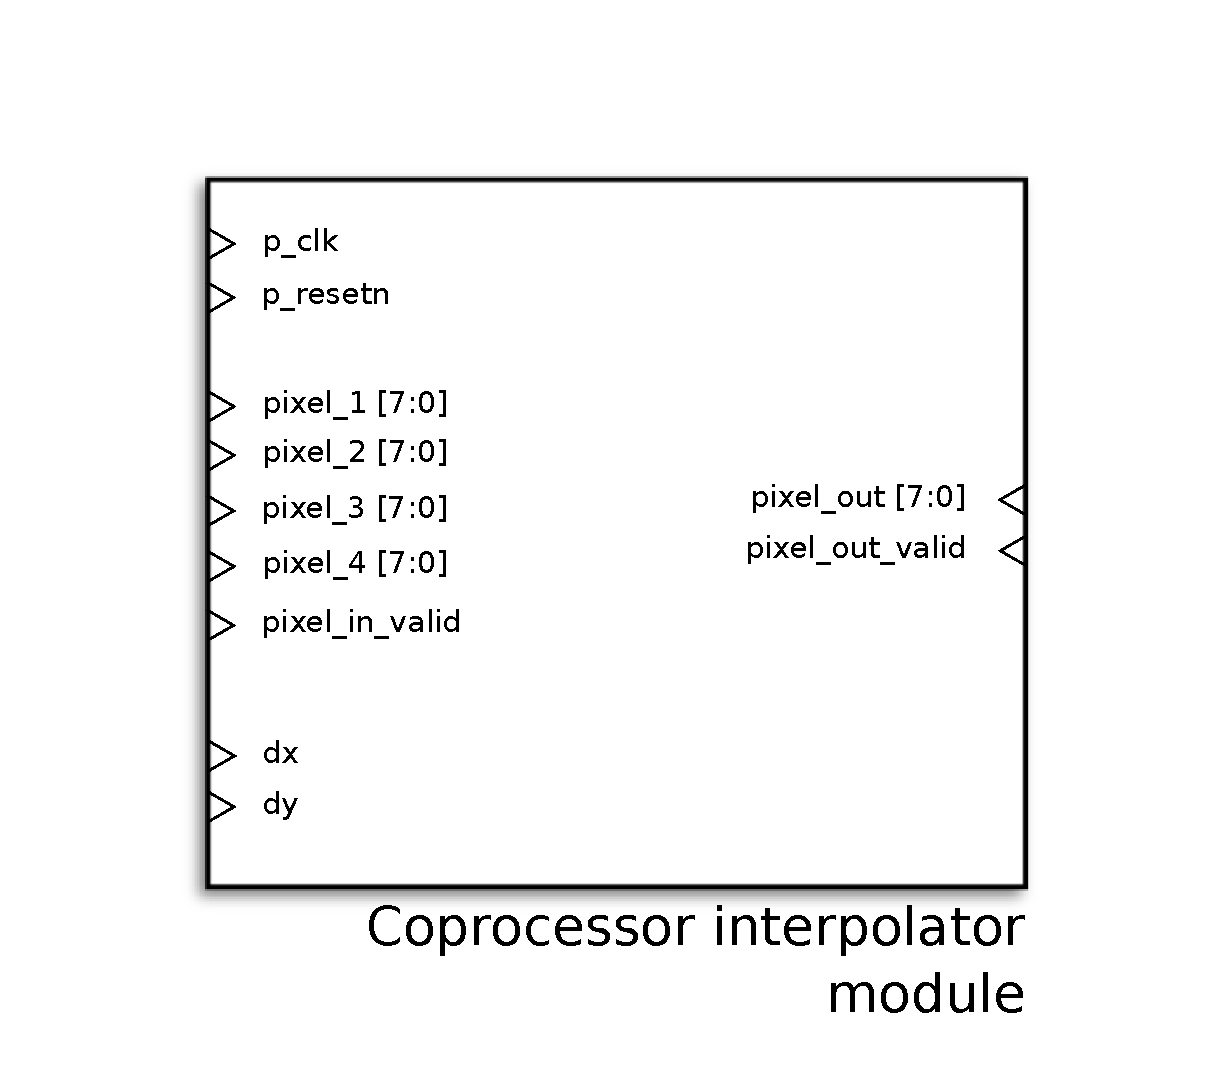
\includegraphics[width=7cm]{figs/INTERPOLATOR.pdf}
\caption{Coprocessor interpolator's interface}
\label{interpo_ports}
\end{figure}



This module consists of a single thread (\texttt{interpolate}) which is responsible for the bilinear interpolation of the fictional pixel. 

On the rising edge of the system clock, and when the input pixels(\texttt{pixel\_0, pixel\_1, pixel\_2, pixel\_3, dx, dy}) are declared as valid (\texttt{pixel\_in\_valid}), the interpolated value is outputted (\texttt{pixel\_out}) along with a signal that defines it's value as valid (\texttt{pixel\_out\_valid}). 
This operation is performed at the rate of 100MHz.  


An alternative implementation that was considered and tested was that of a module that accumulates partial results of the interpolation and creates an outputs pixel at the rate of 25MHz. This architecture is quite convenient since it only requires one inputed pixel at each rising edge of the clock. This fact could lead to a less costly and more compact design of the coprocessor.  

\subsection{Interpolator output module}

\begin{figure}[H]
\center
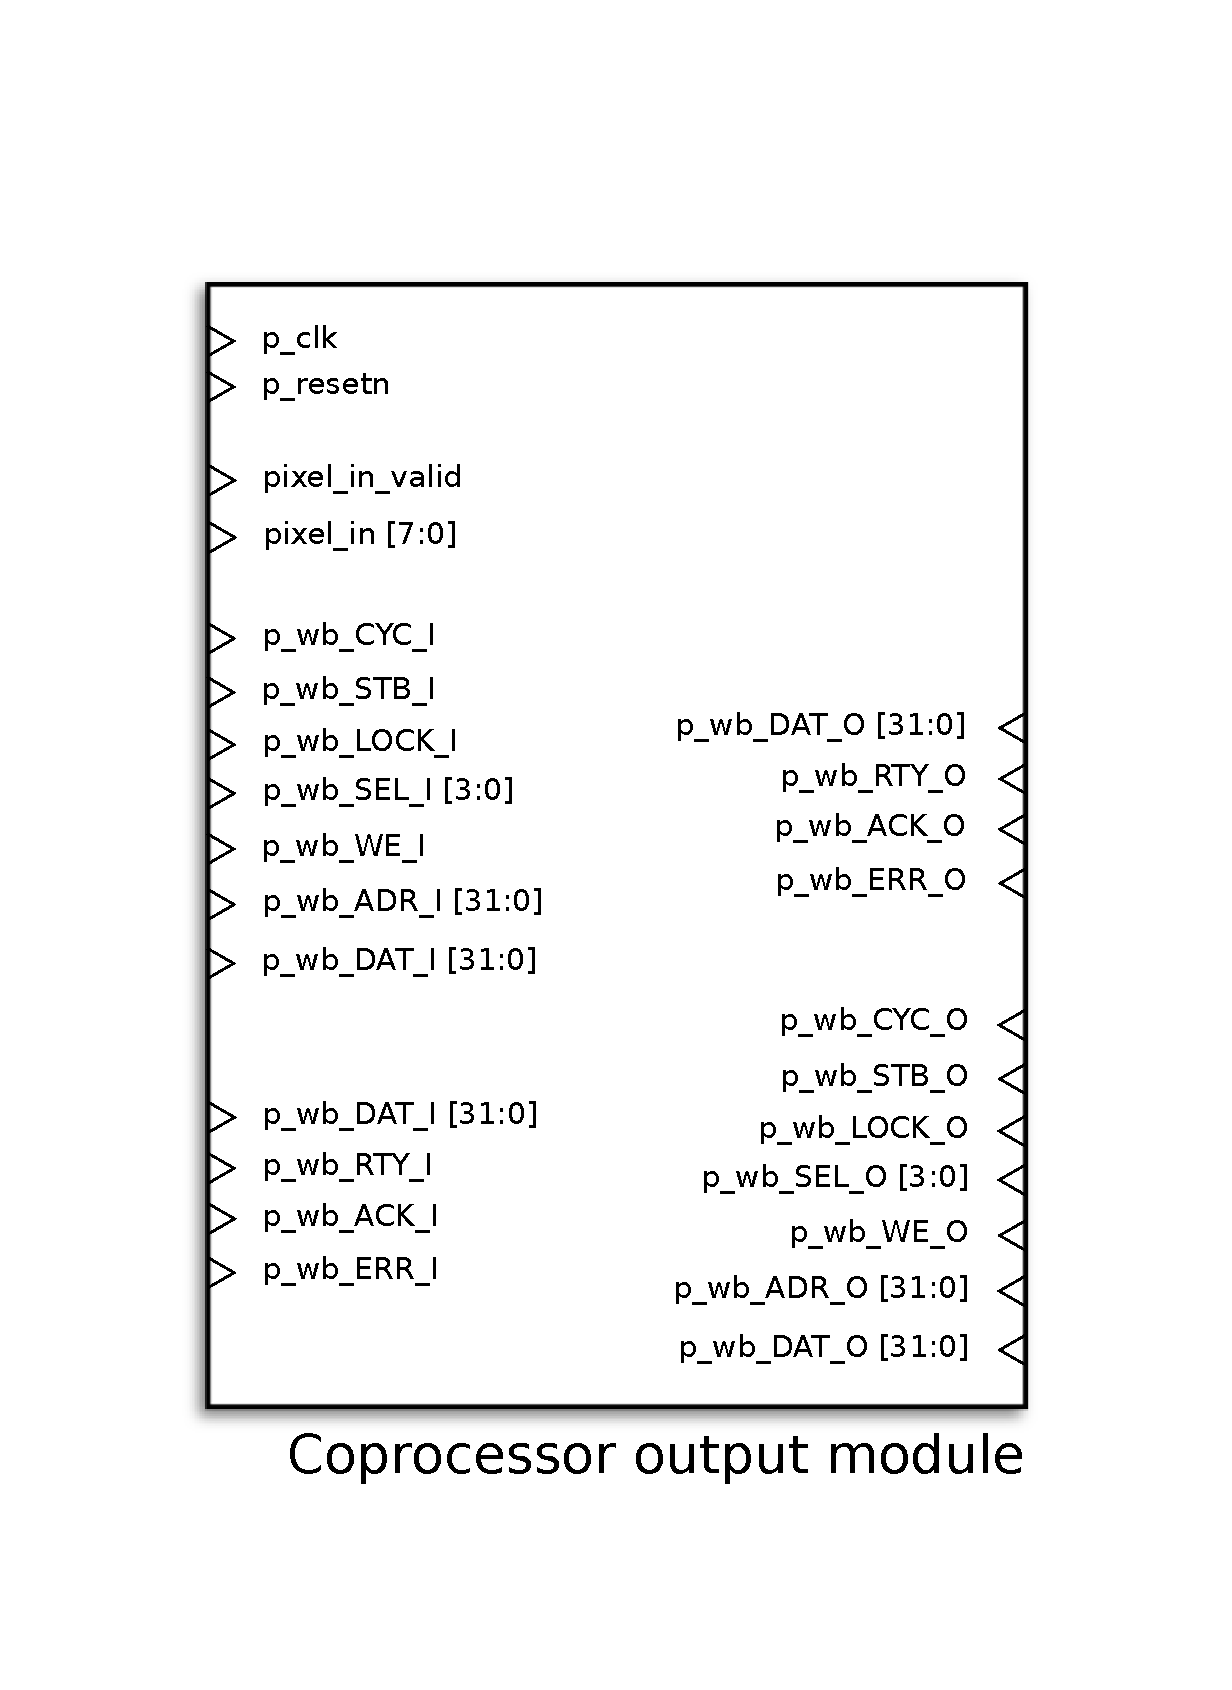
\includegraphics[width=7cm]{figs/INTERPOLATOR_OUT.pdf}
\caption{Coprocessor interpolator out module's interface}
\label{interpo_out_ports}
\end{figure}



The interpolator out module consists of two threads. 

The \texttt{process\_write\_buffer()} thread is responsible of acquiring pixels inputed by the interpolator and storing them in to the local buffer. Pixels inputed to the module (\texttt{pixel\_in}) are stored if the corresponding valid signal is true (\texttt{pixel\_valid}). The \texttt{process\_load\_buffer\_to\_ram()} thread is responsible of storing the locally stored pixels into the RAM. This is done in a tile by tile fashion. The ram memory address in which the image should be saved is stored in a register attached to the wishbone bus and therefore controlled by the processor. 

The \texttt{process\_load\_buffer\_to\_ram} module consults the content of this register once it has finished sending a complete image.

\subsection{Buffer management}

\begin{figure}[H]
\center
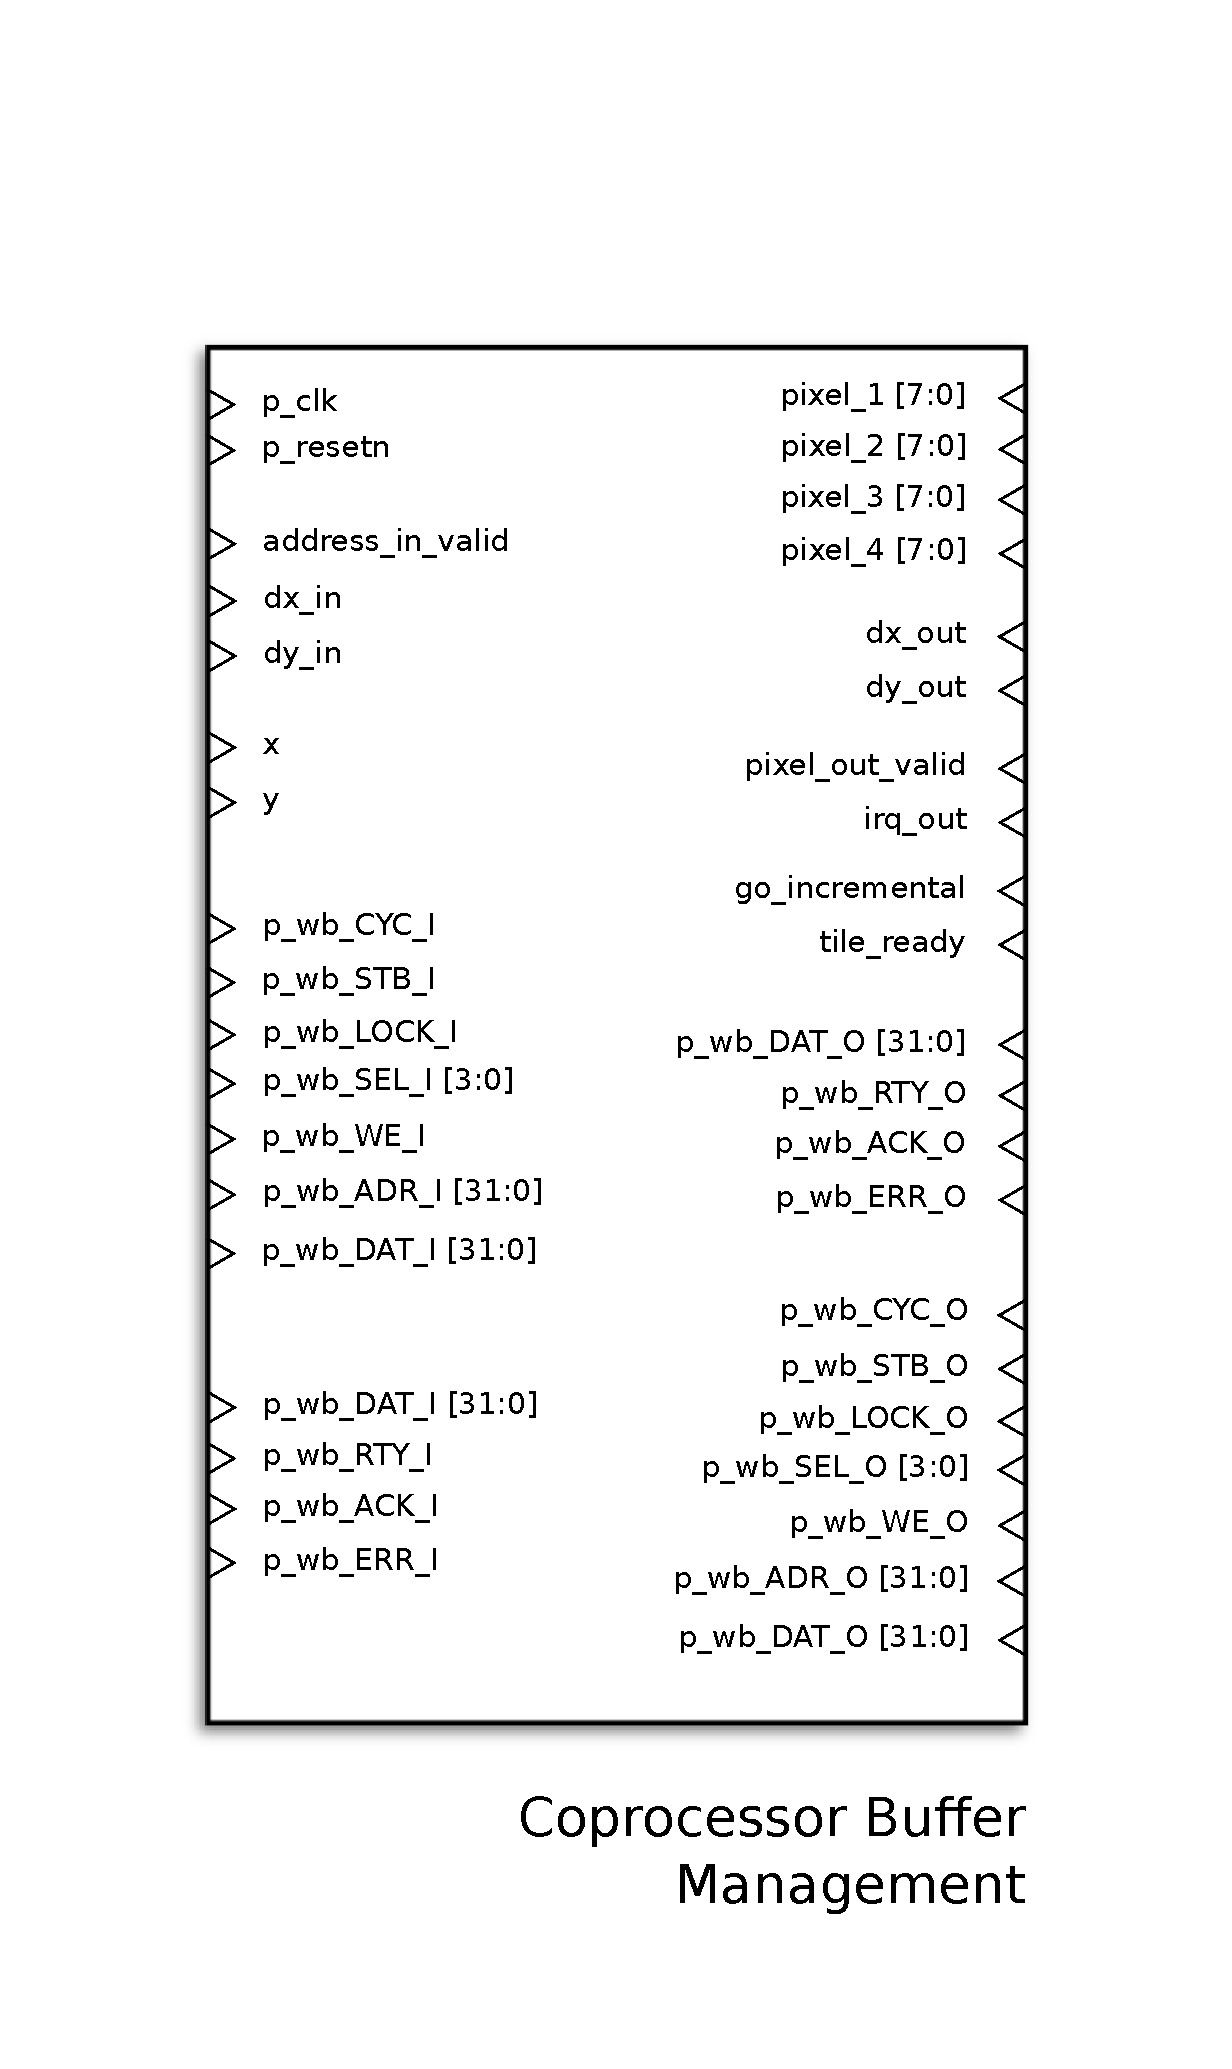
\includegraphics[width=6.9cm]{figs/Buffer_management.pdf}
\caption{Coprocessor buffer management module's interface}
\label{buff_out_ports}
\end{figure}


The \texttt{buffer\_management} module is responsible of loading the local co-processor buffer in a tile by tile fashion and performing the pixel-address to pixel value transformation. The size of the buffer is equal to 2 tiles. At each instant, one part of the buffer is used as a look-up table while the other part is used as storage place for the pre-fetching of the next tile. 

The process \texttt{load\_buffer\_from\_ram} pre-fetches tiles  to be "looked-up". The address of the tile to be pre-fetched is stored in a register attached to the wishbone bus, therefore the processor (LM32) controls the contents of this register. Once the next tile to be "looked-up" has been fetched, this thread consults the content of the register and waits till the current lookup procedure has finished. 

The  \texttt{process\_lookup\_pixel\_intensity}  processor performs the lookup function. Once a tile has been looked up an interrupt is raised notifying therefore the processor. The processor should respond to this interrupt by providing the address of the next tile to be pre-fetched. 

The \texttt{process\_lookup\_pixel\_intensity} process is not allowed to lookup the next tile, unless that tile has been loaded. In this case the incremental calculation module is halted by setting the \texttt{go\_incremental} signal to false.  

%%%%%%%%%%%%%%%%%%%%%%%%%%%%%%%%%%%%%%%%%%%%%%%%%%%%%
%				Mode of Operation					%
%					-----------						%
%													%
% Author: Theodoros Theodoropoulos&Adrian Schindler	%
%%%%%%%%%%%%%%%%%%%%%%%%%%%%%%%%%%%%%%%%%%%%%%%%%%%%%

\section{Mode of operation}

This section regroups all the information detailed in the previous chapters. It summarizes the system on chip's overall mode of operation, and gives some performance details.

\subsection{Summarized mode of operation}

\begin{enumerate}

\item At the start of the system, video generator takes images stored on the disk and starts sending it to \texttt{video\_in} pixel by pixel. The objective of \texttt{video\_in} is to store these pixels on to the ram with the start address specified by LM32. However, at this point \texttt{video\_in} does not have a start address, so it remains Idle until the LM32 performs a write request to \texttt{video\_in}'s embedded slave.

\item After the start address has been written, \texttt{video\_in} waits for a raising edge event of the \texttt{frame\_valid} signal. This will trigger an update of \texttt{video\_in}'s configuration, and will start the video stream transfer.

\item There are two blocks in \texttt{video\_in}. The first one samples the 25Mhz clock (\texttt{Pixel\_in} - interfaced with \texttt{video\_gen}) in order to be synchronized with \texttt{video\_gen}. The second one runs at 100Mhz and is responsible for bus transfers. Once the \texttt{Pixel-in} is given the start signal (which is set only after the first time LM32 has written the destination address), it takes pixels from \texttt{video\_gen} and stores them on to buffer in real time.
Note:- The buffer used here is an array of registers with widow size as 64 bytes. Block size is the number of pixels bytes that will be stored on to the ram as a part of block write. It is here equal to 32.

\item The \texttt{Pixel\_in} block signals the \texttt{Ram\_out} block once it has stored one block of pixels on to the buffer by using the internal \texttt{go} signal. The \texttt{Ram\_out} block will then do a block write of the buffer over the wishbone bus to the ram, and acknowledges the \texttt{Pixel\_in} block using the \texttt{go\_ack} signal

\item At the end of the image, the \texttt{video\_in} module requires a new destination address. Thus, it raises an interrupt on the LM32, which will reply by writing the new configuration to the internal slave. Here again, the configuration is updated at the raising edge of frame valid, so the new address must be transmitted to \texttt{video\_in} between the end of the old frame, and the beginning of the new frame. If this timing is not respected, the old configuration will be used and the older image overwritten. Since the SOC only stores two images, the LM32 sends two different addresses alternatively.

\item The LM32 gives the tile antecedent's address to the coprocessor. Once \texttt{buffer\_management} has raised an interrupt, it responds with the address of the next tile to be pre-fetched. Both processes run in parallel. \texttt{Buffer\_management} reads the internal register \texttt{image\_ready} and loads the pixels into an internal buffer.

\item LM32 also writes the initializations of the variables (s0, s1, ...)  to another slave, with separate addresses for the coefficients of the x and y coordinates. The slave indicates that the initializations are complete by a ready signal (after 40 writes) Similarly, if the coprocessor has read 40 values, the loaded signal indicates this.
Incremental realizes that the load signal is high and loads the register values into internal registers and starts outputting the calculated source coordinates which are then read by the interpolation module.

\item When \texttt{buffer\_management} has loaded the tile, it sets a public register \texttt{tile\_ready} high to indicate the Incremental to start calculating.
\texttt{Buffer\_Management} generates \texttt{Tile\_IRQ} to notify the LM32, and to start loading the next tile (restarts at 3). 
It keeps two buffers: the currently read one and the next one which is pre-loaded for the next 	tile.

\item Once the \texttt{tile\_ready} signal is high, the coprocessor's incremental module starts calculating the transformation with outputs x, y, dx and dy. There is one pixel output for every clock cycle (100 MHz). It should be mentioned that the incremental computation can be switched on and off by the en (enable signal) when for instance the next tile hasn't been pre-fetched yet. This signal is provided by the buffer management module.
One pixel is sent to \texttt{buffer\_management} which also sends one pixel per clock cycle (no latency because the tile has been stored previously into an internal register) to the Interpolation which always takes 1 clock cycle also.
Since the coprocessor only works on a tile-by-tile basis, it outputs a finished signal after 16x16 pixels to show that the calculation has finished.

\item \texttt{Incremental\_Out} runs at 100 MHz and contains the calculated pixel values which are output to \texttt{video\_out}. These pixels are sent in a tile by tile fashion to the Ram through the wishbone bus. The base address of the of the image to be sent to Ram is stored in register connected to the wishbone bus and controlled by the processor. It's value is read when a whole image has been sent to Ram. 

\item \texttt{video\_out} like \texttt{video\_in} has two blocks, one synchronized with the 25Mhz clock (\texttt{Pixel\_out} - interfaced with video display) and the other with the 100Mhz clock (\texttt{Ram\_in}-interfacing wishbone bus).

\item \texttt{video\_out}'s behavior is similar to \texttt{video\_in}'s behavior. It will remain idle until the LM32 gives it the first address to read, and then it will raise an interrupt at the end of every frame to ask for the next frame to read and display. It uses again a buffer to temporarily store pixels from the RAM and give them to video display in real time. 

\end{enumerate}

\subsection{Performance measurements}

To evaluate our current design's performance, we performed the following measurements on the co-simulation(video-in and video-out in system verilog):
\begin{itemize}
\item Initial delay (Time after witch the first image starts to appear on the display) - 32.011ms
\item Time required to write one block to the RAM (32 bytes) - 1150ns.
This includes waiting for the fifo to be read.

\item Standalone write time is 430ns.

\item Time required to read one block from RAM - 1280ns
\item Standalone read time is 520ns

\item Total time for 1 block - 1150+1280\=2430ns

\item Thus, for 1 tile of 16x16 pixels 19440ns\=19.5us approximatively is required.


\end{itemize}

%%%%%%%%%%%%%%%%%%%%%%%%%%%%%%%%%%%%%%%%%%%%%%%%%%%%%
%			    The project's status				%
%					-----------						%
% Author: Thibault Porteboeuf	& Vaibhav Singh		%
%%%%%%%%%%%%%%%%%%%%%%%%%%%%%%%%%%%%%%%%%%%%%%%%%%%%%


\section{Project Status}

\subsection{VideoIn and VideoOut}
Both the modules have been completed in SystemC and System Verilog and have been tested in simulation. The system verilog code is synthesizable (with no warnings and errors). Generic Slave Register has been written in SystemC and Verilog. 

\subsection{Co-Processor}
Co-Processor has buffer management, incremental and interpolator in SystemC. All 3 modules have been individually tested using a test bench. All these modules are connected. Testing needs to be done once the synchronisation with LM32 is completed, which means loading the tile address from the LM32 at a suitable timing. 

\subsection{LM32}
LM32 has interrupt mechanism,Co-Processor Initialisation and Coefficient Calculation for Co-Processor. Code which remains involves writing of the coefficients on Co-Processor's slave registers.

\subsection{conclusion}
Integration and testing of Co-processor in SystemC and then it eventual conversion in System Verilog remains. At start, 3 out of 4 members started with video in and video out code in systemC just to get the feel of the system. In hindsight, we would have liked to start the code of Co-Processor from the day one.



\end{document}
